% !TeX spellcheck = pl_PL
%%%%%%%%%%%%%%%%%%%%%%%%%%%%%%%%%%%%%%%%%%%
%                                        %
% Szablon pracy dyplomowej magisterskiej %
% zgodny  z aktualnymi  przepisami  SZJK %
%                                        %
%%%%%%%%%%%%%%%%%%%%%%%%%%%%%%%%%%%%%%%%%%
%                                        %
%  (c) Krzysztof Simiński, 2018-2023     %
%                                        %
%%%%%%%%%%%%%%%%%%%%%%%%%%%%%%%%%%%%%%%%%%
%                                        %
% Najnowsza wersja szablonów jest        %
% podstępna pod adresem                  %
% github.com/ksiminski/polsl-aei-theses  %
%                                        %
%%%%%%%%%%%%%%%%%%%%%%%%%%%%%%%%%%%%%%%%%%
%
%
% Projekt LaTeXowy zapewnia odpowiednie formatowanie pracy,
% zgodnie z wymaganiami Systemu zapewniania jakości kształcenia.
% Proszę nie zmieniać ustawień formatowania (np. fontu,
% marginesów, wytłuszczeń, kursywy itd. ).
%
% Projekt można kompilować na kilka sposobów.
%
% 1. kompilacja pdfLaTeX
%
% pdflatex main
% bibtex   main
% pdflatex main
% pdflatex main
%
%
% 2. kompilacja XeLaTeX
%
% Kompilatacja przy użyciu XeLaTeXa różni się tym, że na stronie
% tytułowej używany jest font Calibri. Wymaga to jego uprzedniego
% zainstalowania.
%
% xelatex main
% bibtex  main
% xelatex main
% xelatex main
%
%
%%%%%%%%%%%%%%%%%%%%%%%%%%%%%%%%%%%%%%%%%%%%%%%%%%%%%
% W przypadku pytań, uwag, proszę pisać na adres:   %
%      krzysztof.siminski(małpa)polsl.pl            %
%%%%%%%%%%%%%%%%%%%%%%%%%%%%%%%%%%%%%%%%%%%%%%%%%%%%%
%
% Chcemy ulepszać szablony LaTeXowe prac dyplomowych.
% Wypełniając ankietę spod poniższego adresu pomogą
% Państwo nam to zrobić. Ankieta jest całkowicie
% anonimowa. Dziękujemy!


% https://docs.google.com/forms/d/e/1FAIpQLScyllVxNKzKFHfILDfdbwC-jvT8YL0RSTFs-s27UGw9CKn-fQ/viewform?usp=sf_link
%
%%%%%%%%%%%%%%%%%%%%%%%%%%%%%%%%%%%%%%%%%%%%%%%%%%%%%%%%%%%%%%%%%%%%%%%%%

%%%%%%%%%%%%%%%%%%%%%%%%%%%%%%%%%%%%%%%%%%%%%%%
%                                             %
% PERSONALIZACJA PRACY – DANE PRACY           %
%                                             %
%%%%%%%%%%%%%%%%%%%%%%%%%%%%%%%%%%%%%%%%%%%%%%%

% Proszę wpisać swoje dane w poniższych definicjach.

% TODO
% dane autora
\newcommand{\FirstNameAuthor}{inż. Kacper}
\newcommand{\SurnameAuthor}{Nitkiewicz}
\newcommand{\IdAuthor}{290409}   % numer albumu  (bez $\langle$ i $\rangle$)

% drugi autor:
%\newcommand{\FirstNameCoauthor}{Imię}   % Jeżeli jest drugi autor, to tutaj należy podać imię.
%\newcommand{\SurnameCoauthor}{Nazwisko} % Jeżeli jest drugi autor, to tutaj należy podać nazwisko.
%\newcommand{\IdCoauthor}{$\langle$wpisać właściwy$\rangle$}  % numer albumu drugiego autora (bez $\langle$ i $\rangle$)
% Gdy nie ma drugiego autora, należy zostawić poniższe definicje puste, jak poniżej. Gdy jest drugi autor, należy zakomentować te linie.
\newcommand{\FirstNameCoauthor}{} % Jeżeli praca ma tylko jednego autora, to dane drugiego autora zostają puste.
\newcommand{\SurnameCoauthor}{}   % Jeżeli praca ma tylko jednego autora, to dane drugiego autora zostają puste.
\newcommand{\IdCoauthor}{}  % Jeżeli praca ma tylko jednego autora, to dane drugiego autora zostają puste.
%%%%%%%%%%

\newcommand{\Supervisor}{dr inż. Adrian Smagór}     % dane promotora (bez $\langle$ i $\rangle$)
\newcommand{\Title}{Analiza narzędzi wyszukujących zawartość tekstową w systemie Linux}           % tytuł pracy po polsku
\newcommand{\TitleAlt}{Analysis of text search tools in Linux system}                     % thesis title in English
\newcommand{\Program}{Informatyka Przemysłowa}            % kierunek studiów  (bez $\langle$ i $\rangle$)
\newcommand{\Specialisation}{Cyberbezpieczeństwo}     % specjalność  (bez $\langle$ i $\rangle$)
\newcommand{\Departament}{Informatyka Przemysłowa}        % katedra promotora  (bez $\langle$ i $\rangle$)

% Jeżeli został wyznaczony promotor pomocniczy lub opiekun, proszę go/ją wpisać ...
\newcommand{\Consultant}{} % dane promotora pomocniczego, opiekuna (bez $\langle$ i $\rangle$)
% ... w przeciwnym razie proszę zostawić puste miejsce jak poniżej:
%\newcommand{\Consultant}{} % brak promotowa pomocniczego / opiekuna

% koniec fragmentu do modyfikacji
%%%%%%%%%%%%%%%%%%%%%%%%%%%%%%%%%%%%%%%%%%


%%%%%%%%%%%%%%%%%%%%%%%%%%%%%%%%%%%%%%%%%%%%%%%
%                                             %
% KONIEC PERSONALIZACJI PRACY                 %
%                                             %
%%%%%%%%%%%%%%%%%%%%%%%%%%%%%%%%%%%%%%%%%%%%%%%

%%%%%%%%%%%%%%%%%%%%%%%%%%%%%%%%%%%%%%%%

%%%%%%%%%%%%%%%%%%%%%%%%%%%%%%%%%%%%%%%%%%%%%%%
%                                             %
% PROSZĘ NIE MODYFIKOWAĆ PONIŻSZYCH USTAWIEŃ! %
%                                             %
%%%%%%%%%%%%%%%%%%%%%%%%%%%%%%%%%%%%%%%%%%%%%%%



\documentclass[a4paper,twoside,12pt]{book}
\usepackage[utf8]{inputenc}
\usepackage[T1]{fontenc}
\usepackage{amsmath,amsfonts,amssymb,amsthm}
\usepackage[british,polish]{babel}
\usepackage{indentfirst}
\usepackage{xurl}
\usepackage{xstring}
\usepackage{ifthen}
\usepackage{array}

\usepackage{ifxetex}

\ifxetex
    \usepackage{fontspec}
    \defaultfontfeatures{Mapping=tex—text} % to support TeX conventions like ``——-''
    \usepackage{xunicode} % Unicode support for LaTeX character names (accents, European chars, etc)
    \usepackage{xltxtra} % Extra customizations for XeLaTeX
\else
    \usepackage{lmodern}
\fi



\usepackage[margin=2.5cm]{geometry}
\usepackage{graphicx}
\usepackage{hyperref}
\usepackage{booktabs}
\usepackage{tikz}
\usepackage{pgfplots}
\usepackage{mathtools}
\usepackage{geometry}
\usepackage{subcaption}   % subfigures
\usepackage[page]{appendix} % toc,
\renewcommand{\appendixtocname}{Dodatki}
\renewcommand{\appendixpagename}{Dodatki}
\renewcommand{\appendixname}{Dodatek}

\usepackage{csquotes}
\usepackage[natbib=true,backend=bibtex,maxbibnames=99]{biblatex}  % kompilacja bibliografii BibTeXem
%\usepackage[natbib=true,backend=biber,maxbibnames=99]{biblatex}  % kompilacja bibliografii Biberem
\bibliography{biblio/biblio}

\usepackage{ifmtarg}   % empty commands  

\usepackage{setspace}
\onehalfspacing


\frenchspacing

%%%%%%%%%%%%%%%%%%%%%%%%%%%%%%%%%%
% środowiska dla definicji, twierdzenia, przykładu
\usepackage{amsthm}

\newtheorem{Definition}{Definicja}
\newtheorem{Example}{Przykład}
\newtheorem{Theorem}{Twierdzenie}
%%%%%%%%%%%%%%%%%%%%%%%%%%%%%%%%%%

%%%% TODO LIST GENERATOR %%%%%%%%%

\usepackage{color}
\definecolor{brickred}      {cmyk}{0   , 0.89, 0.94, 0.28}

\makeatletter \newcommand \kslistofremarks{\section*{Uwagi} \@starttoc{rks}}
\newcommand\l@uwagas[2]
{\par\noindent \textbf{#2:} %\parbox{10cm}
    {#1}\par} \makeatother


\newcommand{\ksremark}[1]{%
    {%\marginpar{\textdbend}
            {\color{brickred}{[#1]}}}%
    \addcontentsline{rks}{uwagas}{\protect{#1}}%
}

\newcommand{\comma}{\ksremark{przecinek}}
\newcommand{\nocomma}{\ksremark{bez przecinka}}
\newcommand{\styl}{\ksremark{styl}}
\newcommand{\ortografia}{\ksremark{ortografia}}
\newcommand{\fleksja}{\ksremark{fleksja}}
\newcommand{\pauza}{\ksremark{pauza `--', nie dywiz `-'}}
\newcommand{\kolokwializm}{\ksremark{kolokwializm}}
\newcommand{\cudzyslowy}{\ksremark{,,polskie cudzysłowy''}}

%%%%%%%%%%%%%% END OF TODO LIST GENERATOR %%%%%%%%%%%

\newcommand{\printCoauthor}{%		
    \StrLen{\FirstNameCoauthor}[\FNCoALen]
    \ifthenelse{\FNCoALen > 0}%
    {%
        {\large\bfseries\Coauthor\par}

            {\normalsize\bfseries \LeftId: \IdCoauthor\par}
    }%
    {}
}

%%%%%%%%%%%%%%%%%%%%%
\newcommand{\autor}{%		
    \StrLen{\FirstNameCoauthor}[\FNCoALenXX]
    \ifthenelse{\FNCoALenXX > 0}%
    {\FirstNameAuthor\ \SurnameAuthor, \FirstNameCoauthor\ \SurnameCoauthor}%
    {\FirstNameAuthor\ \SurnameAuthor}%
}
%%%%%%%%%%%%%%%%%%%%%

\StrLen{\FirstNameCoauthor}[\FNCoALen]
\ifthenelse{\FNCoALen > 0}%
{%
    \author{\FirstNameAuthor\ \SurnameAuthor, \FirstNameCoauthor\ \SurnameCoauthor}
}%
{%
    \author{\FirstNameAuthor\ \SurnameAuthor}
}%

%%%%%%%%%%%% ZYWA PAGINA %%%%%%%%%%%%%%%
% brak kapitalizacji zywej paginy
\usepackage{fancyhdr}
\pagestyle{fancy}
\fancyhf{}
\fancyhead[LO]{\nouppercase{\it\rightmark}}
\fancyhead[RE]{\nouppercase{\it\leftmark}}
\fancyhead[LE,RO]{\it\thepage}


\fancypagestyle{tylkoNumeryStron}{%
    \fancyhf{}
    \fancyhead[LE,RO]{\it\thepage}
}

\fancypagestyle{bezNumeracji}{%
    \fancyhf{}
    \fancyhead[LE,RO]{}
}


\fancypagestyle{NumeryStronNazwyRozdzialow}{%
    \fancyhf{}
    \fancyhead[LE]{\nouppercase{\autor}}
    \fancyhead[RO]{\nouppercase{\leftmark}}
    \fancyfoot[CE, CO]{\thepage}
}


%%%%%%%%%%%%% OBCE WTRETY  
\newcommand{\obcy}[1]{\emph{#1}}
\newcommand{\english}[1]{{\selectlanguage{british}\obcy{#1}}}
%%%%%%%%%%%%%%%%%%%%%%%%%%%%%

% polskie oznaczenia funkcji matematycznych
\renewcommand{\tan}{\operatorname {tg}}
\renewcommand{\log}{\operatorname {lg}}

% jeszcze jakies drobiazgi

\newcounter{stronyPozaNumeracja}

%%%%%%%%%%%%%%%%%%%%%%%%%%% 
\newcommand{\printOpiekun}[1]{%		

    \StrLen{\Consultant}[\mystringlen]
    \ifthenelse{\mystringlen > 0}%
    {%
        {\large{\bfseries OPIEKUN, PROMOTOR POMOCNICZY}\par}

            {\large{\bfseries \Consultant}\par}
    }%
    {}
}
%
%%%%%%%%%%%%%%%%%%%%%%%%%%%%%%%%%%%%%%%%%%%%%%

% Proszę nie modyfikować poniższych definicji!
\newcommand{\Author}{\FirstNameAuthor\ \MakeUppercase{\SurnameAuthor}}
\newcommand{\Coauthor}{\FirstNameCoauthor\ \MakeUppercase{\SurnameCoauthor}}
\newcommand{\Type}{PRACA MAGISTERSKA}
\newcommand{\Faculty}{Wydział Informatyki Przemysłowej}
\newcommand{\Polsl}{Politechnika Śląska}
\newcommand{\Logo}{graf/politechnika_sl_logo_bw_pion_pl.pdf}
\newcommand{\LeftId}{Nr albumu}
\newcommand{\LeftProgram}{Kierunek}
\newcommand{\LeftSpecialisation}{Specjalność}
\newcommand{\LeftSUPERVISOR}{PROWADZĄCY PRACĘ}
\newcommand{\LeftDEPARTMENT}{KATEDRA}
%%%%%%%%%%%%%%%%%%%%%%%%%%%%%%%%%%%%%%%%%%%%%%

%%%%%%%%%%%%%%%%%%%%%%%%%%%%%%%%%%%%%%%%%%%%%%%
%                                             %
% KONIEC USTAWIEŃ                             %
%                                             %
%%%%%%%%%%%%%%%%%%%%%%%%%%%%%%%%%%%%%%%%%%%%%%%

 % Proszę nie modyfikować pliku settings.tex


%%%%%%%%%%%%%%%%%%%%%%%%%%%%%%%%%%%%%%%%%%%%%%%
%                                             %
% MOJE PAKIETY, USTAWIENIA ITD                %
%                                             %
%%%%%%%%%%%%%%%%%%%%%%%%%%%%%%%%%%%%%%%%%%%%%%%

% Tutaj proszę umieszczać swoje pakiety, makra, ustawienia itd.


 
%%%%%%%%%%%%%%%%%%%%%%%%%%%%%%%%%%%%%%%%%%%%%%%%%%%%%%%%%%%%%%%%%%%%%
% listingi i fragmentu kodu źródłowego 
% pakiet: listings lub minted
% % % % % % % % % % % % % % % % % % % % % % % % % % % % % % % % % % % 

% biblioteka listings
\usepackage{listings}
\lstset{%
morekeywords={string,exception,std,vector},% słowa kluczowe rozpoznawane przez pakiet listings
language=C++,% C, Matlab, Python, SQL, TeX, XML, bash, ... – vide https://www.ctan.org/pkg/listings
commentstyle=\textit,%
identifierstyle=\textsf,%
keywordstyle=\sffamily\bfseries, %\texttt, %
%captionpos=b,%
tabsize=3,%
frame=lines,%
numbers=left,%
numberstyle=\tiny,%
numbersep=5pt,%
breaklines=true,%
escapeinside={@*}{*@},%
}

% % % % % % % % % % % % % % % % % % % % % % % % % % % % % % % % % % % 
% pakiet minted
% \usepackage{minted}

% pakiet wymaga specjalnego kompilowania:
% pdflatex -shell-escape main.tex
% xelatex  -shell-escape main.tex

\usepackage[chapter]{minted} % [section]
%%\usemintedstyle{bw}   % czarno-białe kody 
%
%\setminted % https://ctan.org/pkg/minted
%{
%%fontsize=\normalsize,%\footnotesize,
%%captionpos=b,%
%tabsize=3,%
%frame=lines,%
%framesep=2mm,
%numbers=left,%
%numbersep=5pt,%
%breaklines=true,%
%escapeinside=@@,%
%}

%%%%%%%%%%%%%%%%%%%%%%%%%%%%%%%%%%%%%%%%%%%%%%%%%%%%%%%%%%%%%%%%%%%%%

\usepackage{microtype}
\usepackage{tcolorbox}
\usepackage{pgfplots}
\pgfplotsset{compat=newest}
% \let\cleardoublepage\clearpage

%%%%%%%%%%%%%%%%%%%%%%%%%%%%%%%%%%%%%%%%%%%%%%%
%                                             %
% KONIEC MOICH USTAWIEŃ                       %
%                                             %
%%%%%%%%%%%%%%%%%%%%%%%%%%%%%%%%%%%%%%%%%%%%%%%

 % Tutaj proszę umieścić swoje pakiety, makra, ustawienia itd.

%%%%%%%%%%%%%%%%%%%%%%%%%%%%%%%%%%%%%%%%

\begin{document}
%\kslistofremarks

\frontmatter

%%%%%%%%%%%%%%%%%%%%%%%%%%%%%%%%%%%%%%%%%%%%%%%
%                                             %
% PROSZĘ NIE MODYFIKOWAĆ STRONY TYTUŁOWEJ!    %
%                                             %
%%%%%%%%%%%%%%%%%%%%%%%%%%%%%%%%%%%%%%%%%%%%%%%


%%%%%%%%%%%%%%%%%%  STRONA TYTUŁOWA %%%%%%%%%%%%%%%%%%%
\pagestyle{empty}
{
	\newgeometry{top=1.5cm,%
	             bottom=2.5cm,%
	             left=3cm,
	             right=2.5cm}
 
	\ifxetex 
	  \begingroup
	  \setsansfont{Calibri}
	   
	\fi 
	 \sffamily
	\begin{center}
	\includegraphics[width=50mm]{\Logo}
	 
	
	{\Large\bfseries\Type\par}
	
	\vfill  \vfill  
			 
	{\large\Title\par}
	
	\vfill  
		
	{\large\bfseries\Author\par}
	
	{\normalsize\bfseries \LeftId: \IdAuthor}

	\printCoauthor
	
	\vfill  		
 
	{\large{\bfseries \LeftProgram:} \Program\par} 
	
	{\large{\bfseries \LeftSpecialisation:} \Specialisation\par} 
	 		
	\vfill  \vfill 	\vfill 	\vfill 	\vfill 	\vfill 	\vfill  
	 
	{\large{\bfseries \LeftSUPERVISOR}\par}
	
	{\large{\bfseries \Supervisor}\par}
				
	{\large{\bfseries \LeftDEPARTMENT\ \Departament} \par}
		
	{\large{\bfseries \Faculty}\par}
		
	\vfill  \vfill  

    	
    \printOpiekun{\Consultant}
    
	\vfill  \vfill  
		
    {\large\bfseries  Gliwice \the\year}

   \end{center}	
       \ifxetex 
       	  \endgroup
       \fi
	\restoregeometry
}
  
%%%%%%%%%%%%%%%%%%%%%%%%%%%%%%%%%%%%%%%%%%%%%%%
%                                             %
% KONIEC STRONY TYTUŁOWEJ                     %
%                                             %
%%%%%%%%%%%%%%%%%%%%%%%%%%%%%%%%%%%%%%%%%%%%%%%  
  % Proszę nie modyfikować pliku titlepage.tex

\cleardoublepage

\rmfamily\normalfont
\pagestyle{empty}


%%% No to zaczynamy pisać pracę :-) %%%%

% TODO
\subsubsection*{Tytuł pracy} 
\Title

\subsubsection*{Streszczenie}  
(Streszczenie pracy – odpowiednie pole w systemie APD powinno zawierać kopię tego streszczenia.)

\subsubsection*{Słowa kluczowe} 
(2-5 slow (fraz) kluczowych, oddzielonych przecinkami)

\subsubsection*{Thesis title} 
\begin{otherlanguage}{british}
\TitleAlt
\end{otherlanguage}

\subsubsection*{Abstract} 
\begin{otherlanguage}{british}
(Thesis abstract – to be copied into an appropriate field during an electronic submission – in English.)
\end{otherlanguage}
\subsubsection*{Key words}  
\begin{otherlanguage}{british}
(2-5 keywords, separated by commas)
\end{otherlanguage}

 % informacje redakcyjne


%%%%%%%%%%%%%%%%%% SPIS TRESCI %%%%%%%%%%%%%%%%%%%%%%
% Add \thispagestyle{empty} to the toc file (main.toc), because \pagestyle{empty} doesn't work if the TOC has multiple pages
\addtocontents{toc}{\protect\thispagestyle{empty}}
\tableofcontents

%%%%%%%%%%%%%%%%%%%%%%%%%%%%%%%%%%%%%%%%%%%%%%%%%%%%%
\setcounter{stronyPozaNumeracja}{\value{page}}
\mainmatter
\pagestyle{empty}

\cleardoublepage

\pagestyle{NumeryStronNazwyRozdzialow}

%%%%%%%%%%%%%% wlasciwa tresc pracy %%%%%%%%%%%%%%%%%

% TODO
\chapter{Wstęp}

\section{Wprowadzenie do problemu}
Analiza przeszukiwania struktur danych o dużych rozmiarach z wieloma typami danych stanowi
istotne wyzwanie w dziedzinie inżynierii oprogramowania i zarządzania danymi. 

Jednym ze sposobów zachowywania danych jest archiwizacja plików. Innym 
rozwiązaniem redukującym rozmiar danych jest kompresja. Takie rozwiązanie jest
bardzo przydatne w przypadku chęci
zmniejszenia ilości danych przechowywanych, a także w dystrybucji danych dla
innych użytkowników.

Otrzymana biblioteka jako zbiór książek i dokumentów była przekazana do analizy.
Celem przekazania było wykonanie odszukań tekstu w zbiorze i zlokalizowania
ścieżki pliku, znalezionego tekstu.

W kwestii technicznej należało rozważyć sposób efektywnego zarządzania pamięcią
w przypadku czytania dużej ilości danych z dysku, jak i opóźnienia związane z 
wydajnością operacji I/O.

Problem wyszukiwania danych nastąpił w momencie wyszukiwania dużej ilości 
zawartości danych. Oryginalne archiwum zajmuje 15 GB danych, gdzie pliki są 
zarchiwizowane, co utrudnia odczytanie z nich danych. 

Wykonanie operacji odczytu archiwów będzie miało kluczowe znaczenie w 
otrzymaniu informacji o miejscu znajdowania się treści, choć może znacznie 
wpłynąć na kompleksowość rozwiązania \cite{bib:ksiazka:kompleksowośćArchiwów}.

Implementacja poznanych algorytmów pozwoliła na określenie, który algorytm 
optymalnie wyszukuje zawartość w wykorzystywanym zbiorze danych. A niewielkie
różnice sposobu odczytu danych wpływały na prędkość wydajność wyszukania.

Dodatkowo odczytywanie archiwów w archiwach wymaga kilkukrotnego wyodrębnienia
danych. Aby otrzymać odpowiednią ilość wyników, należy wyodrębnić 
wszystkie zagnieżdżone archiwa. Zasadniczo archiwa po wydobyciu,
tworzą drzewo plików, w którym mogą znajdować się kolejne archiwa, z kolejnym drzewem
plików itd. Odczytanie zawartości odbędzie się poprzez przejście po drzewie 
każdego z wyodrębnionego archiwum.

\section{Cel Pracy}

Celem niniejszej pracy jest analiza algorytmów wyszukujących zawartość tekstową 
w standardzie ASCII oraz ocena ich efektywności w systemie operacyjnym Linux. 
Kluczowym zagadnieniem badawczym jest porównanie różnych metod przeszukiwania 
tekstu pod względem szybkości działania oraz dokładności. Skupiono się na 
implementacjach tych algorytmów w języku programowania Golang, który oferuje
rozbudowane narzędzia testujące i profilujące kod.

Praca ma na celu nie tylko teoretyczne zestawienie wybranych algorytmów, ale 
także ich praktyczną implementację i porównanie w rzeczywistym środowisku 
obliczeniowym. W tym kontekście istotnym aspektem jest zbadanie wydajności 
różnych podejść do przeszukiwania tekstu w dużych zbiorach danych, w tym w 
archiwach z zagnieżdżonymi folderami.

Kolejnym celem jest ocena poprawności działania zaimplementowanych algorytmów, 
co oznacza sprawdzenie, czy znajdują one wszystkie wystąpienia szukanych fraz w 
sposób zgodny z oczekiwaniami. W szczególności badane będą przypadki graniczne, 
takie jak wyszukiwanie w dużych plikach, przeszukiwanie czy analiza wpływu 
długości wzorca na czas wyszukiwania.

Ostatecznym celem pracy jest dostarczenie rekomendacji dotyczących wyboru 
odpowiedniego algorytmu wyszukiwania tekstowego w zależności od specyfiki 
zadania. Analiza porównawcza umożliwi wskazanie rozwiązań optymalnych pod 
względem wydajności oraz zastosowania w różnych warunkach systemowych.

\section{Zakres Pracy}
Zakres pracy obejmuje szczegółową analizę algorytmów wyszukiwania tekstu w Golang.
W pierwszej części pracy przedstawione zostaną teoretyczne podstawy algorytmów wyszukiwania,
w tym klasyczne podejścia, takie jak algorytm Knutha-Morrisa-Pratta, Boyera-
Moore'a oraz inne techniki wyszukiwania w tekście ASCII.

Kolejnym etapem będzie implementacja wybranych algorytmów w języku Golang oraz 
ich optymalizacja pod kątem wydajności. Przeprowadzone zostaną testy porównawcze, 
w których oceniana będzie szybkość wyszukiwania oraz skuteczność w znajdowaniu
wzorców tekstowych. Dodatkowo uwzględniona zostanie analiza wpływu wielkości
pliku oraz długości wzorca na efektywność działania poszczególnych metod.

Praca obejmuje również testowanie wydajności algorytmów w rzeczywistym 
środowisku systemu Linux. Badania będą prowadzone w konsolowym interfejsie 
użytkownika, gdzie zaimplementowane algorytmy zostaną przetestowane na 
rzeczywistych zbiorach archiwalnych. Zostaną również porównane czasy wykonania
wyszukiwania w zależności od długości frazy.

Na zakończenie pracy zostaną zaprezentowane wyniki przeprowadzonych badań wraz 
z wnioskami dotyczącymi efektywności analizowanych algorytmów. Na podstawie 
uzyskanych wyników zostaną sformułowane rekomendacje dotyczące stosowania 
poszczególnych metod wyszukiwania tekstowego w zależności od rodzaju danych 
oraz wymagań wydajnościowych.

% \textbf{TODO opis ogólny rozdziałów} 
% \begin{itemize}
% \item wprowadzenie w problem/zagadnienie 
%\item osadzenie problemu w dziedzinie 
%\item cel pracy 
%\item zakres pracy 
%\item zwięzła charakterystyka rozdziałów 
% \end{itemize}

  % wstęp

% TODO
\chapter{Analiza tematu wyszukiwania tekstu}  % Analiza tematu
% 

%\begin{itemize}
%\item Jaki problem chcę (muszę :-) rozwiązać?
%\item Dlaczego rozwiązanie problemu jest ważne?
%\item Jak inni rozwiązują ten problem?
%\item Jakie są zalety i wady tych rozwiązań?
%\end{itemize}

%Odwołania do literatury:
%książek \cite{bib:ksiazka},
%artykułów w czasopismach \cite{bib:artykul},
%materiałów konferencyjnych \cite{bib:konferencja}
%i stron www \cite{bib:internet}.
%
%Równania powinny być numerowane
\begin{align}
    y = \frac{\partial x}{\partial t}
\end{align}


\begin{itemize}
\item analiza tematu
\item wprowadzenie do dziedziny (\english{state of the art}) – sformułowanie problemu, 
\item poszerzone studia literaturowe, przegląd literatury tematu (należy wskazać źródła wszystkich informacji zawartych w pracy)
\item opis znanych rozwiązań, algorytmów, osadzenie pracy w kontekście
\item Tytuł rozdziału jest często zbliżony do tematu pracy. 
\item Rozdział jest wysycony cytowaniami do literatury \cite{bib:artykul,bib:ksiazka,bib:konferencja}. 
Cytowanie książki \cite{bib:ksiazka}, artykułu w czasopiśmie \cite{bib:artykul}, artykułu konferencyjnego \cite{bib:konferencja} lub strony internetowej \cite{bib:internet}.
\end{itemize}

%\begin{Definition}\label{def:1}
%Definicja to zdanie (lub układ zdań) odpowiadające na pytanie o strukturze „co to jest a?”. Definicja normalna jest zdaniem złożonym z 2 członów: definiowanego (łac. definiendum) i definiującego (łac. definiens), połączonych spójnikiem definicyjnym („jest to”, „to tyle, co” itp.). 
%\end{Definition}
%
%\begin{Theorem}[Pitagorasa]\label{t:pitagoras}
%W dowolnym trójkącie prostokątnym suma kwadratów długości przyprostokątnych jest równa kwadratowi długości przeciwprostokątnej tego trójkąta. 
%\end{Theorem}
%
%\begin{Example}[generalizacja]\label{ex:generalizacja}
%Przykładem generalizacji jest para: zwierzę i pies. Pies jest zwierzęciem. Pies jest uszczegółowieniem pojęcia zwierzę. Zwierzę jest uogólnieniem pojęcia pies.
%\end{Example}
\section{Sformułowanie problemu}
Wyszukiwanie tekstu w systemach towarzszy ludziom od początków istnienia maszyn,
choć pierwsze komputery nie posiadały ogromnych ilość pamięci co nie powodowało
potrzeby istnienia algorytmów wyszukujących tekst. Procesor Intel 8008 
zaprezentowany w 1972 posiadał jedynie 14 bitową magistrale adresową co 
pozwalało na 16 Kbi pamięci. Model Motoroli 68000 posiada 5 MB dysku twardego,
co nie może się równać z opecnym standardem darmowej pamięci udostępnianej w 
chmurze przez Google (15 GB).

Problem wyszukiwania danych nastąpił w momencie tworzenia dużej ilość zawartości.
Posiadane archiwum wynosi 14.7 GB danych, niektóre z zawartości są 
zarchiwizowane co znacznie utrudnia odczytania z nich danych. Nie mniej jednak,
posiadane narzędzia w systemach dają dużą dowolność w wyszukania zawartości,
która nas interesuje.

Zasadniczym problem naszej pracy jest wyszukiwanie zawartości tekstowej
ogramnej ilość plików w różnych formatach. Takie podejście może okazać się 
problematyczne w przypadku plików dzwiękowych, filomowych czy zdjęć wszelkiego
rodzaju.

\section{State of art}

Podjęcie problemu wyszukiwania plików po nazwach oraz zawartości jest bardzo
złożonym i trudnym problemem w sferze programistycznej. Istnieje wiele rozwiązań
tego problemu, które istnieją od początku pracy z komputerem. Narzędzia takie
jak \textbf{find}, grep czy fzf \cite{bib:internet:Fzf} pozwalają na wyszukiwanie
zawartości która nas interesuje, ale kompleksowość tych narzędzi nie jest 
przystosowana do tak trudnego problemu, jakim jest wyszukiwanie treści w plikach,
które są zarchiwizowane. Z taką samą niedogodnością spotykamy się w przypadku
plików pochodzących z pakietu Microsoft Office 365, jednak jeśli rozwiążemy 
zadanie otrzymywania zawartości z archiwów, będziemy w stanie otrzymać również 
zawartość z plików z rozszerzeniami .doc, .docx czy .pptx.

Narzędzie \textbf{find} to znane i popularne narzędzie wśród osób zaznajomionych z
technologiami linuxowymi. Już bardzo często wykorzystywany do znajdowania plików
w systemie, jednak nie nadaje sie do znajdowania zawartości plików.

\begin{figure}[h]
  \centering
  \begin{lstlisting}
# Find files by extension:
    find root_path -name '*.ext'

# Find files matching multiple path/name patterns:
    find root_path -path '**/path/**/*.ext' -or -name '*pattern*'

# Find directories matching a given name, in case-insensitive mode:
    find root_path -type d -iname '*lib*'

# Find files matching a given pattern, excluding specific paths:
    find root_path -name '*.py' -not -path '*/site-packages/*'

# Find files matching a given size range, limiting the recursive depth to "1":
    find root_path -maxdepth 1 -size +500k -size -10M

# Run a command for each file (use `{}` within the command to access the filename):
    find root_path -name '*.ext' -exec wc -l {} \;

# Find all files modified today and pass the results to a single command as arguments:
    find root_path -daystart -mtime -1 -exec tar -cvf archive.tar {} \+

# Find empty (0 byte) files and delete them:
    find root_path -type f -empty -delete
  \end{lstlisting}
  \caption{Przykłady użycia programu find}
  \label{fig:code:bashFindExamples}
\end{figure}

Do przeszukiwania zawartości plików dobrze nadaje się narzędzie grep, który jest
dostępny w każdej dystrybucji Linuxa. Jego działanie jest dość podobne do finda,
lecz posiada on możliwość wyszukiwania treść w plikach tekstowych jak również
archiwach. Nie posiada on niestety możliwość szukania zawartości plików .pdf oraz
nie wspiera formatów książkowych takich jak .djvu.

\begin{figure}[h]
  \centering
  \begin{lstlisting}
# Search for a pattern within a file:
    grep "search_pattern" path/to/file

# Search for an exact string (disables regular expressions):
    grep -F|--fixed-strings "exact_string" path/to/file
sec
# Search for a pattern in all files recursively in a directory, showing line numbers of matches, ignoring binary files:
    grep -r|--recursive -n|--line-number --binary-files without-match "search_pattern" path/to/directory

# Use extended regular expressions (supports `?`, `+`, `{}`, `()` and `|`), in case-insensitive mode:
    grep -E|--extended-regexp -i|--ignore-case "search_pattern" path/to/file

# Print 3 lines of context around, before, or after each match:
    grep --context|before-context|after-context 3 "search_pattern" path/to/file

# Print file name and line number for each match with color output:
    grep -H|--with-filename -n|--line-number --color=always "search_pattern" path/to/file

# Search for lines matching a pattern, printing only the matched text:
    grep -o|--only-matching "search_pattern" path/to/file

# Search `stdin` for lines that do not match a pattern:
    cat path/to/file | grep -v|--invert-match "search_pattern"
  \end{lstlisting}
  \caption{Przykłady użycia programu grep}
  \label{fig:code:bashGrepExamples}
\end{figure}

Istnieje również ripgrep, który jest sukcesorem wcześniej wymienionego
narzędzia. Jego wydajność przewyższa grepa nawet trzydziestokrotnie w niektórych
testach sprawnościowych, jednak zazwyczaj jest to niewielki wzrost. Nie jest on
niestety domyślnie instalowany na większości systemów linuxowych. Nie posiada on
również wsparcia dla formatów pdf i djvu.

Można wyszukiwać również po treści piosenek, ale wymagałoby to utworzenie modelu
sztucznej inteligencji, która wydobywałaby tekst z piosenek do postaci tekstowej.

%%%%%%%%%%%%%%%%%%%%%%%%%%%%%%%%%%%%%%%%%%%%%%%%%%%%%%%%%%%%%%%%%%%%%%%%%%%%%%%%
\section{Opis poznanych rozwiązań}
\subsection{Algorytm brute force}

Jest wiele algorytmów, które wyszukują tekst. Jednym z takich algorytmów jest 
algorytm typu brute-force. Polega sprawdzaniu każdego bajtu, jego implementacja
jest bardzo prosta i standardowa, a złożoność czasowe tego rozwiązania wynosi
O(m * n), gdzie m to długość bloku (pattern), a n to długość tekstu (substring),
którego szukamy. 

\begin{figure}[h]
  \centering
  \begin{lstlisting}
for i := 0; i<len(pattern); i++{
  for j := 0; j<len(substring); j++{
    // compare bytes
  }
}
  \end{lstlisting}
  \caption{Przykłady algorytmu brute force}
  \label{fig:code:bruteForceComparison}
\end{figure}

Zaletą tego algorytmu jest to, że nie posiada potrzeby przechowywać żadnych 
danych w pamięci. Ten algorytm dobrze sprawdza się gdy posiadamy ograniczoną 
ilość zasobów pamięci, co nie jest problemem w obecnych czasach, gdy pamięć jest
stosunkowo tania i szeroko dostępna.
\begin{figure}[h]
  \centering
  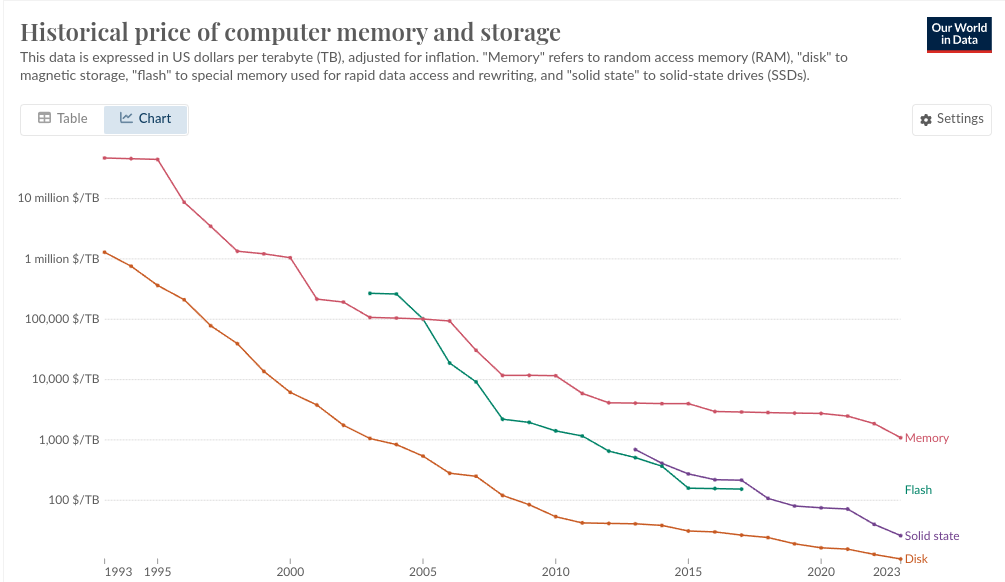
\includegraphics[width=0.9\textwidth]{./images/historical-mem-price.png}
  \caption{Historyczne dane cen pamięci w latach 1993-2023 }
  \label{screenshot:MemPrices}
\end{figure}
%\cite{internet:HistoricalMemPrice}
%https://jcmit.net/memoryprice.htm

Powyższy algorytm można zrównoleglić, dzieląc wzorzec na mniejsze części
i wyszukując tylko dane w tym obszarze, ale należy dołożyć końce wzorca, aby nie
wynikła sytuacja, w której wzorzec by wystąpił, ale nie wzięto pod uwagę końca 
zdania. 

\begin{center}
  \begin{tabular}{ |c|c|  } 
    \hline
    \multicolumn{2}{|c|}{TYTUL} \\
    \hline
    wzorzec & ABCABCABDABD \\
    \hline
    podłańcuch & BCA \\
    \hline
    rezultat & 4 \\
    \hline
  \end{tabular}
\end{center}

Jeżeli podzielimy wzorzec na dwa procesy wyszukujące algorytmem brute-force,
otrzymamy dwa zadania:

\begin{center}
  \begin{tabular}{ |c|c||c|c|  } 
    \hline
    \multicolumn{4}{|c|}{Zadania} \\
    \hline
    Zadanie 1 & & Zadanie 2 & \\
    \hline
    wzorzec & ABCABC & wzorzec & ABDABD \\
    \hline
    podłańcuch & BCA & podłańcuch & BCA \\
    \hline
    rezultat & -1 & rezultat & -1 \\ 
    \hline
  \end{tabular}
\end{center}

Zrównoleglenie procesu powoduje, że otrzymaliśmy nie poprawny wynik, gdyż w 
żadnym z wzorców nie występuje podłańcuch "BCA", choć łańcuch występuje w 
miejscu 4, to algorytm nie posiada wiedzy o dalszej części wzorca.

Aby poprawić dany algorytm należy dołożyć znaki, które należy sprawdzać w 
przypadku poprawnego rozpatrzenia ostatniego znaku.


\begin{center}
  \begin{tabular}{ |c|c||c|c|  } 
    \hline
    \multicolumn{4}{|c|}{Zadania} \\
    \hline
    Zadanie 1 & & Zadanie 2 & \\
    \hline
    wzorzec & ABCABC(AB) & wzorzec & ABDABD(nil) \\
    \hline
    podłańcuch & BCA & podłańcuch & BCA \\
    \hline
    rezultat & 4 & rezultat & -1 \\ 
    \hline
  \end{tabular}
\end{center}

W takim przypadku sprawdzamy tylko do sytuacji, w której BC jest częścią
podłańcucha, ale podłańcuch nie został w pełni znaleziony. Długość ponownego 
wyszukania byłaby równa len(podłańcuch) - 1.

\subsection{Algorytm Morisa-Pratta}

Algorytm Morisa-Pratta jest dość prostym algorytmem wykorzystującym możliwość
wcześniejszego sprocesowania podłańcucha wyszukiwanego w tekście co przyspiesza
sposób procesowania tekstu. Polega on na wykorzystaniu faktu istnienia pasującego
prefikso sufiksu. Pozwala to na pominięcie pewnych porównania niektórych znaków,
bez szkody w wyniku wyszukiwania.

Dzięki wykorzystaniu tej zależności możemy uniknąć cofania się indeksu i. 
Tablice preproc wypełniamy poprzednią wartości tak długo aż zaistnieje różnica 
pomiędzy obecnym a następnym znakiem tablicy substr. W przypadku różnicy 
zwiększamy wartość zapisywaną do tablicy preprocesora o odległość różnicy znaków.
W ten sposób następnym razem będzie możliwość pominięcia porównania tych znaków.

\begin{figure}[h]
  \centering
  \begin{lstlisting}
curr = -1
preproc[0] = -1
for i := 1; i <= len(substr); i++ {
  for (curr > -1) && (substr[curr] != substr[i-1]) {
    curr = preproc[curr]
  }
  curr++
  preproc[i] = curr
}
  \end{lstlisting}
  \caption{Przykład preprocesowania podłańcucha }
  \label{fig:code:preprocessMorisPratt}
\end{figure}

W drugim etapie można wykorzystać wcześniej przygotowaną tablice przemieszczeń 
\textbf{preproc}, aby obliczyć ilość przesunięcia w przypadku znalezienia 
niepasującego prefiksu. Dzięki temu zwykle dłuższy tekst znajdujący się w 
\textbf{s} możemy przeanalizować szybciej niż w przypadku algorytmu bruteforce.
Powoduje to niestety problem w przypadku, gdy napis w którym wyszukujemy nie 
jest wystarczająco długi.

\begin{figure}[h]
  \centering
  \begin{lstlisting}
res := []int{}
curr := 0
found := 0
for i := 0; i < len(s); i++ {
  for (curr > -1) && (substr[curr] != s[i]) {
    curr = preproc[curr]
  }
  curr++
  if curr == len(substr) {
    for found < i-curr+1 {
      found++
    }
    res = append(res, found)
    found++
    curr = preproc[curr]
  }
}
  \end{lstlisting}
  \caption{Przykład preprocesowania podłańcucha }
  \label{fig:code:preprocessMorisPratt}
\end{figure}

W podstawowej bibliotece języka Golang, w pakiecie \textit{strings} istnieje 
implementacja metody \textit{Index()}. Nie jest ona jednak w pełni przedstawiona
w kodzie, natomiast w jej implementacji można zauważyć, że algorytm brute force
jest wykorzystywany tylko w przypadku gdy długość wzorca wynosi więcej niż 64.

\begin{figure}[h]
  \centering
  \begin{lstlisting}
func Index(s, substr string) int {
  n := len(substr)
	switch {
	case n == 0:
		return 0
  [...]
	case n > len(s):
		return -1
	case n <= bytealg.MaxLen: // Zwykle ten case
		// Use brute force when s and substr both are small
		if len(s) <= bytealg.MaxBruteForce /* 64 */{
			return bytealg.IndexString(s, substr)
		}
  [...]
  }
}
  \end{lstlisting}
  \caption{ Szukanie łańcucha w standardowej bibliotece Golang }
  \label{fig:code:preprocessMorisPratt}
\end{figure}

W przypadku w go gdy wzorzec jest większy niż 64 to wykonuje się algorytm 
podobny do Morisa-Pratta, który jednak posiada dodatkową walidacje w przypadku
odkrycia false positives. Algorytm Morisa-Pratta nie potrzebuje takiej walidacji.
 % [Analiza tematu]

% TODO
\chapter{Przedmiot pracy - Wybór najlepszego rozwiązania wyszukiwania tekstu
pod względem wydajności}

%\begin{itemize}
%  \item  Jak ja rozwiązuję problem?
%  \begin{itemize}
%    \item rozwiązanie zaproponowane przez dyplomanta
%    \item analiza teoretyczna rozwiązania
%    \item uzasadnienie wyboru zastosowanych metod, algorytmów, narzędzi
%  \end{itemize}
%\end{itemize}

\section{Rozwiązanie zaproponowane przez dyplomanta}

Przed wyborem metody sprawdzającej należy wykonać heurystyke danych. Jest to 
wymagane, ponieważ wydajność algorytmu jest ściśle powiązana z danymi, które
będziemy przeszukiwać. Jeżeli większość danych, które analizujemy mają charakter
tekstowy, to lepszym rozwiązaniem będzie skorzystanie z ostatniego algorytmu
\ref{sch:algoBoyerMoore}, jednak w innym przypadku warto wykorzystać jeden z 
pozostałych.

Do tego zadania należałoby przeznaczyć narzędzia, które dobrze sobie radzą z 
taką analizą. 

\begin{itemize}
  \item duc
  \item rclone
  \begin{enumerate}
    \item ls 
    \item ncdu
  \end{enumerate}
  \item tree
  \begin{enumerate}
    \item tree -h --du | wc -l -> 14307
    \item tree -h --du -> 13827 files, 481 dirs
  \end{enumerate}
  \item skomplikowane połączenie komend
  \begin{verbatim}
find . -type f -exec file --mime-type {} \; |
awk -F': ' '{print $2}' |
sort |
uniq -c |
sort -nr
  \end{verbatim}
\end{itemize}

\begin{table}[h]
    \centering
    \begin{tabular}{lr}
        \hline
        \textbf{Typ MIME} & \textbf{Ilość} \\
        \hline
        image/jpeg & 5,303 \\
        text/html & 2,473 \\
        image/gif & 2,353 \\
        text/xml & 1,233 \\
        application/pdf & 656 \\
        application/postscript & 488 \\
        text/plain & 285 \\
        application/x-java-applet & 270 \\
        application/zip & 153 \\
        text/x-c & 134 \\
        application/gzip & 126 \\
        text/x-c++ & 121 \\
        text/csv & 64 \\
        application/octet-stream & 56 \\
        text/x-java & 49 \\
        application/x-rar & 34 \\
        application/x-tar & 9 \\
        application/x-dosexec & 3 \\
        application/msword & 3 \\
        text/x-diff & 2 \\
        inode/x-empty & 2 \\
        application/x-compress-ttcomp & 2 \\
        application/vnd.openxmlformats-officedocument.wordprocessingml.document & 2 \\
        application/vnd.ms-cab-compressed & 2 \\
        application/vnd.microsoft.portable-executable & 2 \\
        application/mac-binhex40 & 2 \\
        application/x-ms-ne-executable & 1 \\
        application/x-msaccess & 1 \\
        application/x-ace-compressed & 1 \\
        \hline
    \end{tabular}
    \caption{Dystrybucja w danych na podstawie typu plików MIME}
    \label{tabela:typyMIMEdataset}
\end{table}
% TODO GO FROM HERE

Wykorzystanie kilku znanych algorytmów do przeszukiwania zawartości
tekstu i sprawdzenie, który z nich najlepiej sprawdza się pod względem prędkości
i dokładności wyszukiwania. 

Program nie ma na celu modyfikować informacji zawartych w plikach w żaden sposób.
Powoduje to, że zostaną sprawdzane w statyczny sposób z co spowoduje zasadniczą
regularność i spójność w wynikach danego algorytmu na tych samych danych.

Innym sposobem na rozwiązanie problemu jest wykorzystanie dostępnych narzędzi i
dostosowanie ich do problemu, który rozwiązujemy. Takie rozwiązanie może okazać
się szybsze jeżeli zależy nam na uzyskaniu rezultatu natomiast istnieje 
prawdopodobieństwo wykorzystania narzędzia nieodpowiedniego do danego problemu.

\section{Uzasadnienie wyboru zastosowanych metod, algorytmów, narzędzi}
Do utworzenia programu wykorzystam nowoczesny język programowania Golang \cite{bib:internet:golang}.
Posiada on bardzo wygodny model współbierzności programu co może okazać się 
kluczowe w przypadku tego rodzaju problemu. Dodatkowym plusem tego języka jest
to, że jego składnia jest bardzo czytelna i wzorująca na prostocie początkowych
kompilowanych języków programowania (C).
%TODO make benchmarks on real data

%%%%%%%%%%%%%%%%%%%%%%%%%%%%%%%%%%%%%%%%%%%%%%%%%%%%%%%%%%%%%%%%%%%%%%%%%%%%%%%%
W całym dokumencie powinny znajdować się odniesienia do zawartych w nim ilustracji (rys. \ref{fig:2}).
\begin{figure}
\centering
\begin{tikzpicture}
\begin{axis}[
    y tick label style={
        /pgf/number format/.cd,
            fixed,   % po zakomentowaniu os rzednych jest indeksowana wykladniczo
            fixed zerofill, % 1.0 zamiast 1
            precision=1,
        /tikz/.cd
    },
    x tick label style={
        /pgf/number format/.cd,
            fixed,
            fixed zerofill,
            precision=2,
        /tikz/.cd
    }
]
\addplot [domain=0.0:0.1] {rnd};
\end{axis} 
\end{tikzpicture}
\caption{Wykres przebiegu funkcji.} % Podpis jest zawsze POD rysunkiem.
\label{fig:2}
\end{figure}


%%%%%%%%%%%%%%%%%%%%%
%% RYSUNEK Z PLIKU
%
%\begin{figure}
%\centering
%
\includegraphics[width=0.5\textwidth]{./graf/politechnika_sl_logo_bw_pion_pl.pdf}
%\caption{Podpis rysunku zawsze pod rysunkiem.}
%\label{fig:etykieta-rysunku}
%\end{figure}
%Rys. \ref{fig:etykieta-rysunku} przestawia …
%%%%%%%%%%%%%%%%%%%%%
%
%%%%%%%%%%%%%%%%%%%%%
%% WIELE RYSUNKÓW 
%
%\begin{figure}
%\centering
%\begin{subfigure}{0.4\textwidth}
%    
\includegraphics[width=\textwidth]{./graf/politechnika_sl_logo_bw_pion_pl.pdf}
%    \caption{Lewy górny rysunek.}
%    \label{fig:lewy-gorny}
%\end{subfigure}
%\hfill
%\begin{subfigure}{0.4\textwidth}
%    
\includegraphics[width=\textwidth]{./graf/politechnika_sl_logo_bw_pion_pl.pdf}
%    \caption{Prawy górny rysunek.}
%    \label{fig:prawy-gorny}
%\end{subfigure}
%
%\begin{subfigure}{0.4\textwidth}
%    
\includegraphics[width=\textwidth]{./graf/politechnika_sl_logo_bw_pion_pl.pdf}
%    \caption{Lewy dolny rysunek.}
%    \label{fig:lewy-dolny}
%\end{subfigure}
%\hfill
%\begin{subfigure}{0.4\textwidth}
%    
\includegraphics[width=\textwidth]{./graf/politechnika_sl_logo_bw_pion_pl.pdf}
%    \caption{Prawy dolny rysunek.}
%    \label{fig:prawy-dolny}
%\end{subfigure}
%        
%\caption{Wspólny podpis kilku rysunków.}
%\label{fig:wiele-rysunkow}
%\end{figure}
%Rys. \ref{fig:wiele-rysunkow} przestawia wiele ważnych informacji, np. rys. \ref{fig:prawy-gorny} jest na prawo u góry.
%%%%%%%%%%%%%%%%%%%%%


Tekst dokumentu powinien również zawierać odniesienia do tabel (tab. \ref{id:tab:wyniki}).

\begin{table}
\centering
\caption{Opis tabeli nad nią.}
\label{id:tab:wyniki}
\begin{tabular}{rrrrrrrr}
\toprule
	         &                                     \multicolumn{7}{c}{metoda}                                      \\
	         \cmidrule{2-8}
	         &         &         &        \multicolumn{3}{c}{alg. 3}        & \multicolumn{2}{c}{alg. 4, $\gamma = 2$} \\
	         \cmidrule(r){4-6}\cmidrule(r){7-8}
	$\zeta$ &     alg. 1 &   alg. 2 & $\alpha= 1.5$ & $\alpha= 2$ & $\alpha= 3$ &   $\beta = 0.1$  &   $\beta = -0.1$ \\
\midrule
	       0 &  8.3250 & 1.45305 &       7.5791 &    14.8517 &    20.0028 & 1.16396 &                       1.1365 \\
	       5 &  0.6111 & 2.27126 &       6.9952 &    13.8560 &    18.6064 & 1.18659 &                       1.1630 \\
	      10 & 11.6126 & 2.69218 &       6.2520 &    12.5202 &    16.8278 & 1.23180 &                       1.2045 \\
	      15 &  0.5665 & 2.95046 &       5.7753 &    11.4588 &    15.4837 & 1.25131 &                       1.2614 \\
	      20 & 15.8728 & 3.07225 &       5.3071 &    10.3935 &    13.8738 & 1.25307 &                       1.2217 \\
	      25 &  0.9791 & 3.19034 &       5.4575 &     9.9533 &    13.0721 & 1.27104 &                       1.2640 \\
	      30 &  2.0228 & 3.27474 &       5.7461 &     9.7164 &    12.2637 & 1.33404 &                       1.3209 \\
	      35 & 13.4210 & 3.36086 &       6.6735 &    10.0442 &    12.0270 & 1.35385 &                       1.3059 \\
	      40 & 13.2226 & 3.36420 &       7.7248 &    10.4495 &    12.0379 & 1.34919 &                       1.2768 \\
	      45 & 12.8445 & 3.47436 &       8.5539 &    10.8552 &    12.2773 & 1.42303 &                       1.4362 \\
	      50 & 12.9245 & 3.58228 &       9.2702 &    11.2183 &    12.3990 & 1.40922 &                       1.3724 \\
\bottomrule
\end{tabular}
\end{table}  

 % [Przedmiot pracy]

% TODO
\chapter{Badania}

 

%Rozdział przedstawia przeprowadzone badania. Jest to zasadnicza część i~musi wyraźnie dominować w~pracy.
%Badania i analizę wyników należy przeprowadzić, tak jak jest przyjęte w środowisku naukowym (na przykład korzystanie z danych benchmarkowych, walidacja krzyżowa, zapewnienie powtarzalności testów itd). 
%
%\section{Metodyka badań}
%
%\begin{itemize}
%\item opis metodyki badań
%\item opis stanowiska badawczego (opis interfejsu aplikacji badawczych -- w~załączniku)
%\end{itemize}
%
%
%\section{Zbiory danych}
%
%\begin{itemize}
%\item opis danych
%\end{itemize}
%
%
%\section{Wyniki}
%
%\begin{itemize}
%\item prezentacja wyników, opracowanie i poszerzona dyskusja  wyników, wnioski
%\end{itemize}
%
% 
%\begin{table}
%\centering
%\caption{Opis tabeli nad nią.}
%\label{id:tab:wyniki}
%\begin{tabular}{rrrrrrrr}
%\toprule
%	         &                                     \multicolumn{7}{c}{metoda}                                      \\
%	         \cmidrule{2-8}
%	         &         &         &        \multicolumn{3}{c}{alg. 3}        & \multicolumn{2}{c}{alg. 4, $\gamma = 2$} \\
%	         \cmidrule(r){4-6}\cmidrule(r){7-8}
%	$\zeta$ &     alg. 1 &   alg. 2 & $\alpha= 1.5$ & $\alpha= 2$ & $\alpha= 3$ &   $\beta = 0.1$  &   $\beta = -0.1$ \\
%\midrule
%	       0 &  8.3250 & 1.45305 &       7.5791 &    14.8517 &    20.0028 & 1.16396 &                       1.1365 \\
%	       5 &  0.6111 & 2.27126 &       6.9952 &    13.8560 &    18.6064 & 1.18659 &                       1.1630 \\
%	      10 & 11.6126 & 2.69218 &       6.2520 &    12.5202 &    16.8278 & 1.23180 &                       1.2045 \\
%	      15 &  0.5665 & 2.95046 &       5.7753 &    11.4588 &    15.4837 & 1.25131 &                       1.2614 \\
%	      20 & 15.8728 & 3.07225 &       5.3071 &    10.3935 &    13.8738 & 1.25307 &                       1.2217 \\
%	      25 &  0.9791 & 3.19034 &       5.4575 &     9.9533 &    13.0721 & 1.27104 &                       1.2640 \\
%	      30 &  2.0228 & 3.27474 &       5.7461 &     9.7164 &    12.2637 & 1.33404 &                       1.3209 \\
%	      35 & 13.4210 & 3.36086 &       6.6735 &    10.0442 &    12.0270 & 1.35385 &                       1.3059 \\
%	      40 & 13.2226 & 3.36420 &       7.7248 &    10.4495 &    12.0379 & 1.34919 &                       1.2768 \\
%	      45 & 12.8445 & 3.47436 &       8.5539 &    10.8552 &    12.2773 & 1.42303 &                       1.4362 \\
%	      50 & 12.9245 & 3.58228 &       9.2702 &    11.2183 &    12.3990 & 1.40922 &                       1.3724 \\
%\bottomrule
%\end{tabular}
%\end{table}  
%
%\begin{figure}
%\centering
%\begin{tikzpicture}
%\begin{axis}[
%    y tick label style={
%        /pgf/number format/.cd,
%            fixed,   % po zakomentowaniu os rzednych jest indeksowana wykladniczo
%            fixed zerofill, % 1.0 zamiast 1
%            precision=1,
%        /tikz/.cd
%    },
%    x tick label style={
%        /pgf/number format/.cd,
%            fixed,
%            fixed zerofill,
%            precision=2,
%        /tikz/.cd
%    }
%]
%\addplot [domain=0.0:0.1] {rnd};
%\end{axis} 
%\end{tikzpicture}
%\caption{Podpis rysunku po rysunkiem.}
%\label{fig:2}
%\end{figure}
%
%
%\begin{figure}
%\begin{lstlisting}
%if (_nClusters < 1)
%	throw std::string ("unknown number of clusters");
%if (_nIterations < 1 and _epsilon < 0)
%	throw std::string ("You should set a maximal number of iteration or minimal difference -- epsilon.");
%if (_nIterations > 0 and _epsilon > 0)
%	throw std::string ("Both number of iterations and minimal epsilon set -- you should set either number of iterations or minimal epsilon.");
%\end{lstlisting}
%\caption{Przykład pseudokodu}
%\end{figure}


\section{Metodyka badań}

\subsection{Cel badania}

Celem badani jest sprawdzenie wydajności algorytmów wyszukujących na zbiorze
danych dostarczonego w celu wyszukania treści.

\subsection{Zakres badania}

Zakres badań obejmuje porównanie prędkości algorytmów w celu ustalenia, który
z nich jest najszybszy pod względem czasu wykonania. Zostanie to ustalone na
mniejszym zbiorze rozpakowanych archiwów. Następnie na pełnym zbiorze archiwów
zostanie wykonane porównanie narzędzi pod względem liczby wyszukań oraz prędkości
wyszukań.

\subsection{Hipoteza badań}

Hipotezą badań jest to, że kolejne algorytmy będą wykonywały się szybciej niż ich
poprzednicy. Hipotezą pomocniczą jest to, iż im większy zbiór informacji zebrany
na podstawie łańcucha szukanego tym większa prędkość algorytmu. Dodatkową hipotezą jest
to, iż wykorzystanie \english{Garbage Collectora} wpływa na stabilność 
otrzymywanych wyników.

% \section{Sposób przeprowadzenia badań}
\section{Badanie benchmarku algorytmów}

\begin{figure}[h]
  \centering
  \begin{lstlisting}
go test -test.bench=. -benchmem . -benchtime=1x -count=10

func BenchmarkMorisPrattWindowWord(b *testing.B) {
	var founds = []string{}
	mp := &MorisPratt{}
	filepath.Walk(DIR, WalkAndFindByAlgo(mp,
    &founds, []byte("window")))
	if len(founds) != 11598 {
		b.Fatal("test failed", len(founds), 11598)
	}
}
  \end{lstlisting}
  \caption{Przykład wykonania testu benchmarkowego}
  \label{fig:code:examplePerfTest}
\end{figure}
Badanie zostało przeprowadzone na maszynie autora, podczas działania środowiska
graficznego na Fedora 40. Procesor wykonujący operacje to Intel Core i7-6700K
w architekturze amd64.

Przeprowadzenie badań polegało na uruchomieniu komendy w pierwszej linii (rys. 
\ref{fig:code:examplePerfTest}) i wykonaniu funkcji na algorytmie Morisa Pratta. 
Wykonano testy na wyszukaniu 3 słów, które mogły występować w zbiorze danych,
ze względu na wcześniej przeanalizowaną zawartość. Tymi słowami były 
\textit{"window"}, \textit{"function"}, \textit{"main"}.


\textit{"founds"} jest zmienną przechowującą miejsce znalezionego 
ciągu wyszukiwanego, a mp to struktura przechowująca implementacje algorytmu oraz
bufor wcześniejszego procesowania dla ciągu wyszukiwanego. Pierwsza implementacja nie 
posiadała tej struktury i bufor wcześniejszego procesowania był obliczany przy każdym 
przebiegu algorytmu. To znacznie wpłynęło na prędkość działania algorytmu 
Boyera-Moora.

\begin{Definition}\label{def:WalkFuncGolang}
WalkFunc jest to typ funkcji przyjmowany przez funkcje Walk w module filePath.
Funkcja ta przyjmuje 3 argumenty: ścieżkę, informacje o analizowanym pliku oraz
argument przyjmujący błąd i zwraca błąd. \newline \newline
\textit{type WalkFunc func(path string, info fs.FileInfo, err error) error}
\end{Definition}

W linijce 6 (rys. \ref{fig:code:examplePerfTest}) wykonujemy Przejście (ang. 
\english{Walk}) po drzewie plików w \textit{DIR}, który posiada ścieżkę do 
zbioru danych oraz przyjmuje funkcje zdefiniowaną jako WalkFunc 
\ref{def:WalkFuncGolang}. Z powodu potrzeby czytania tylko zawartości plików,
wykorzystaliśmy funkcje WalkAndFindByAlgo, która będzie czytała pliki, ale 
pozwoli algorytmom podanym w argumencie na przeszukanie zawartości w celu 
znalezienia słowa \textit{"window"}. Po zakończeniu funkcji Walk otrzymano 
tablice znalezionych \textbf{founds}, wypełnioną miejscami, w których wystąpiło znalezienie podanego
ciągu. W liniach 8-10 każdy test posiada walidacje, aby wszystkie wyniki 
otrzymane przez algorytm, były zgodne.

\begin{figure}[h]
  \centering
  \begin{lstlisting}
goos: linux
goarch: amd64
pkg: github.com/gadzbi123/algorytmy/regular
cpu: Intel(R) Core(TM) i7-6700K CPU @ 4.00GHz
BenchmarkMorisPrattFunction-8 1	1041257510 ns/op 264623392 B/op 198976 allocs/op
BenchmarkMorisPrattFunction-8 1	1043653365 ns/op 264645080 B/op 198994 allocs/op
BenchmarkMorisPrattFunction-8 1	1040809273 ns/op 264632096 B/op 198971 allocs/op
BenchmarkMorisPrattFunction-8 1	1043999476 ns/op 264656192 B/op 199008 allocs/op
BenchmarkMorisPrattFunction-8 1	1047795718 ns/op 264641272 B/op 199006 allocs/op
BenchmarkKurtMorisPrattFunction-8 1	1059705156 ns/op 264679568 B/op 199007 allocs/op
BenchmarkKurtMorisPrattFunction-8 1	1044558720 ns/op 264704264 B/op 199016 allocs/op
BenchmarkKurtMorisPrattFunction-8 1	1069466845 ns/op 264722128 B/op 199032 allocs/op
BenchmarkKurtMorisPrattFunction-8 1	1062064344 ns/op 264666880 B/op 199024 allocs/op
BenchmarkKurtMorisPrattFunction-8 1	1062586497 ns/op 264697544 B/op 199018 allocs/op
BenchmarkBoyerMooreFunction-8 1	1163758449 ns/op 264251408 B/op 193795 allocs/op
BenchmarkBoyerMooreFunction-8 1	1142778080 ns/op 264249440 B/op 193831 allocs/op
BenchmarkBoyerMooreFunction-8 1	1127766499 ns/op 264255336 B/op 193817 allocs/op
BenchmarkBoyerMooreFunction-8 1	1169790667 ns/op 264177232 B/op 193775 allocs/op
BenchmarkBoyerMooreFunction-8 1	1128862027 ns/op 264270616 B/op 193811 allocs/op
  \end{lstlisting}
  \caption{Przykładowy rezultat performance}
  \label{fig:perfTestResults}
\end{figure}
W rezultacie wykonania otrzymujemy dane o czasie przebiegu funkcji, ilości 
alokacji oraz ile bajtów wykorzystano na operacje (rys. \ref{fig:perfTestResults}).

\subsection{Zbiór badań}
\begin{table}[h]
    \centering
    \begin{tabular}{|l|l|l|}
        \hline
        \textbf{Typ MIME} & \textbf{Rozmiar (w KB)} & \textbf{Ilość} \\
        \hline
application/pdf & 1094989.16 & 656 \\
application/zip & 911563.68 & 153 \\
application/x-rar & 751425.98 & 34 \\
application/gzip & 158709.61 & 126 \\
application/postscript & 151226.98 & 488 \\
text/html & 49879.89 & 2473 \\
image/jpeg & 49342.96 & 5303 \\
image/gif & 42260.80 & 2353 \\
text/xml & 16914.17 & 1233 \\
application/x-tar & 10470.00 & 9 \\
application/mac-binhex40 & 4704.44 & 2 \\
text/plain & 2929.91 & 285 \\
application/octet-stream & 2131.61 & 56 \\
application/ms.portable-executable & 1552.50 & 2 \\
application/x-ms-ne-executable & 1404.35 & 1 \\
text/x-c++ & 1139.31 & 121 \\
application/x-ace-compressed & 1004.49 & 1 \\
application/msword & 460.50 & 3 \\
application/x-compress-ttcomp & 362.78 & 2 \\
text/x-c & 332.51 & 134 \\
application/x-java-applet & 293.44 & 270 \\
application/x-msaccess & 154.00 & 1 \\
application/x-dosexec & 117.99 & 3 \\
text/x-java & 94.38 & 49 \\
application/vnd.ms-cab-compressed & 88.34 & 2 \\
text/csv & 54.14 & 64 \\
text/x-diff & 46.94 & 2 \\
application/wordprocessingml.document & 34.65 & 2 \\
text/x-script.python & 1.90 & 1 \\
inode/x-empty & 0.00 & 2 \\
Total & 3253691.41 & 13831 \\
        \hline
    \end{tabular}
    \caption{Ilość danych na podstawie typu MIME}
    \label{tabela:typy-MIME-z-iloscia}
\end{table}
%application/zip                               9312014.35 KB      236
%audio/mpeg                                    2771693.64 KB      541
%application/x-rar                             1358304.96 KB       31
%application/vnd.ms-htmlhelp                    337207.65 KB      100
%application/octet-stream                       302676.00 KB       71
%image/jpeg                                     228285.10 KB     1347
%video/x-ms-asf                                 223755.41 KB       15
%image/vnd.djvu                                 174702.98 KB       24
%application/postscript                          84778.60 KB      442
%application/x-ace-compressed                    83686.03 KB        3
%application/gzip                                72011.68 KB       58
%image/gif                                       38853.47 KB     1622
%text/html                                       38485.94 KB     1788
%application/msword                              29155.00 KB       75
%audio/ogg                                       24242.73 KB       25
%application/x-tar                               20940.00 KB       18
%application/x-dosexec                            9318.01 KB        2
%audio/x-wav                                      9180.17 KB        1
%application/x-bzip2                              6383.85 KB        5
%text/rtf                                         4710.93 KB        2
%application/mac-binhex40                         4704.44 KB        2
%text/x-c++                                       4021.66 KB      347
%video/x-msvideo                                  3731.00 KB        1
%application/vnd.ms-powerpoint                    3420.50 KB        1
%text/x-c                                          987.73 KB      345
%text/plain                                        858.96 KB      136
%text/x-tex                                        748.25 KB       64
%application/winhelp                               216.03 KB        1
%application/pdf                                   112.13 KB        1
%image/x-portable-greymap                           54.24 KB        5
%text/x-diff                                        45.52 KB        2
%application/x-matlab-data                          40.19 KB        1
%message/rfc822                                     31.62 KB        1
%text/xml                                           23.51 KB        1
%application/x-shockwave-flash                      21.97 KB        1
%application/x-ole-storage                          20.00 KB        1
%application/x-winhelp                              16.43 KB        1
%text/x-makefile                                    10.37 KB        7
%image/x-xfig                                        7.15 KB        3
%application/javascript                              6.91 KB        1
%application/x-wine-extension-ini                    2.53 KB        4
%text/x-perl                                         1.92 KB        1
%inode/x-empty                                       0.00 KB       20
%Total                                         15149469.59 KB     7353

Zbiór danych (tab. \ref{tabela:typy-MIME-z-iloscia}) posiadał znaczną ilość plików pdf, które w niektórych przypadkach
można było odczytać. Gdy pdf został stworzony z dokumentu tekstowego takiego
jak docx czy odt, to zawartość tekstowa została zawarta w dokumencie pdf. Jeżeli
natomiast pdf został stworzony ze skanu książki, nie zapisała się treść tekstowa.
Wtedy cała treść jest przechowana w postaci zdjęcia, które nie można odczytać użytym
rozwiązaniem.

Możliwość odczytania zawartości daje narzędzie OCR (ang. \english{Optical Character Recognition}).
Narzędzie może służyć do oczytania zawartości plików pdf oraz tekstu z obrazów.
Takie rozwiązanie nie zostanie użyte w pracy, gdyż nie skupiamy się tu na 
algorytmach sztucznej inteligencji.

Pliki audio to piosenki oraz podcasty, których nie można łatwo odczytać algorytmem.
Do oczytania treści z takich plików można wykorzystać narzędzia dokonujące 
trankrypcji, czyli konwersujące rozpoznaną mowę na tekst, jednak te rozwiązania bazują 
na sztucznej inteligencji.

Kolejnym problemem okazało się odczytanie plików formatu doc, które są starym 
formatem dokumentów wykorzystywanych przez Microsoft i ich zakodowana treść nie
jest łatwa do odczytu. W odróżnieniu od formatu docx, który jest archiwum, 
narzędzie nie podejmie się odczytania plików doc. Z uwagi na to, że archiwum danych
jest dość stare, nie wystąpiły tam dokumenty formatu docx. Gdyby wystąpił można
by odczytać zawartość archiwów docx w ten sam sposób jak w przypadku innych 
archiwów.

Archiwa, które są analizowane też trudno odczytać, gdyż stosowane są różne 
rozszerzenia np. zip, rar, 7z, tar. To powoduje, że należy wykorzystać wiele
metod konwersji tych plików do faktycznej struktury możliwej do odczytania. 
Biblioteka, którą wykorzystano nie obsługuje plików skompresowanych przez gzip.
To powoduje, że pliki z rozszerzeniem .gz nie będą otwierane.

Pobrane archiwa posiadały brakujące dane i to powodowało, że biblioteka konwertująca
archiwa miała problem z ich otwarciem. Z tego powodu część danych musiała być 
pominięta, aby program nie został przerwany przez SEGV. Wykorzystana biblioteka
musiała zostać niepoprawnie zaimplementowana, gdyż istnieją programy umiejące 
otworzyć te archiwa, choć nie wszystkie z tych narzędzi działały poprawnie. 

\begin{figure}
\centering
\begin{subfigure}{0.7\textwidth}
    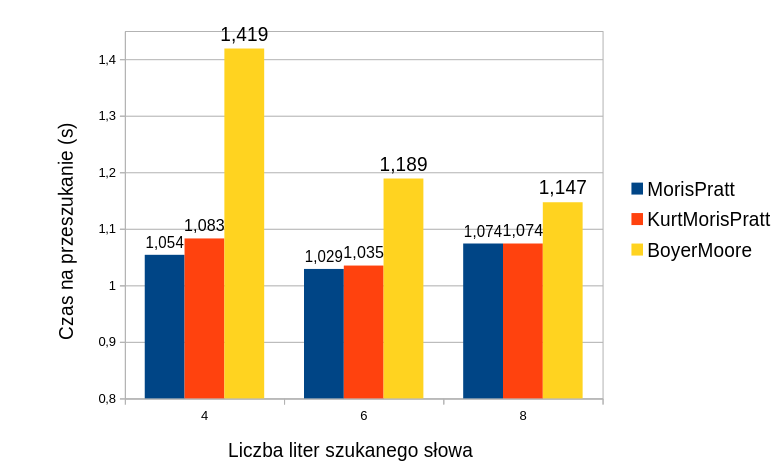
\includegraphics[width=\textwidth]{./images/GraphFirstAttempt.png}
    \caption{Wykres czasów bez statycznego bufora pliku oraz z ponowną 
    rekalkujacją bufora pre-procesora.}
    \label{fig:GraphFirstAttempt}
\end{subfigure}
%\hfill
\begin{subfigure}{0.7\textwidth}
    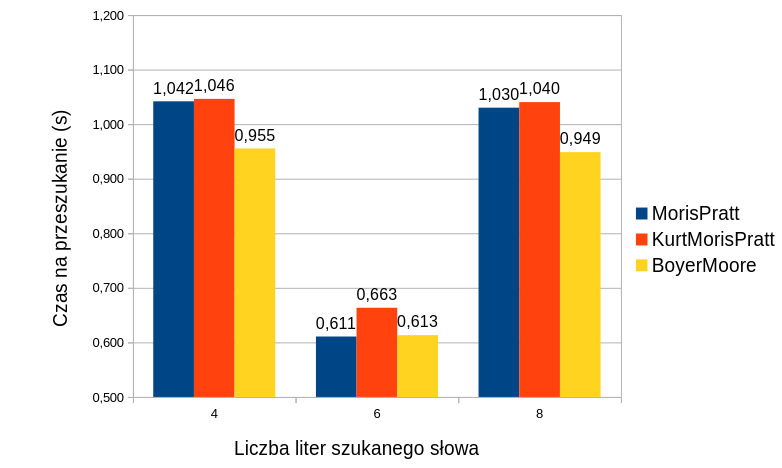
\includegraphics[width=\textwidth]{./images/GraphPreAllocBM.png}
    \caption{Wykres czasów bez statycznego bufora pliku z jednokrotną kalkulacją
     bufora pre-procesora dla algorytmu Boyer Moore'a. }
    \label{fig:GraphPreAllocBM}
\end{subfigure}
\begin{subfigure}{0.7\textwidth}
    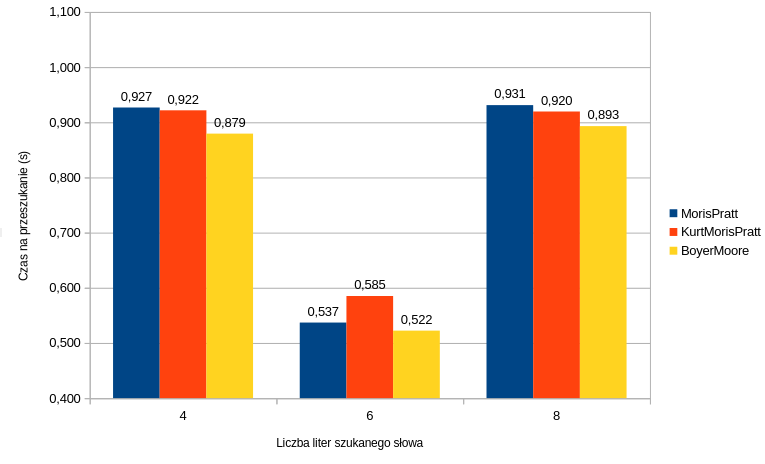
\includegraphics[width=\textwidth]{./images/GraphStaticPreallocAndFileBuffer.png}
    \caption{Wykres czasów z statycznym buforem pliku oraz statycznym buforem
    pre-procesora dla każdego algorytmu.}
    \label{fig:GraphStaticPreallocAndFileBuffer}
\end{subfigure}
\caption{Wykresy kolejnych iteracji na algorytmach}
\label{fig:GraphsIterationComparison}
\end{figure}

Pierwszy test wydajnościowy, który został przeprowadzony, sprawdzał wszystkie 
foldery, w których znajdowały się pliki. Za drugim razem ograniczono się tylko
do plików, które mogą posiadać oczekiwaną zawartość, odrzucając zatem część 
plików ze zbioru. Wykonano testy na 3 algorytmach, gdzie odczytywano 5191 plików 
i łącznie 240 MB danych. Oto rezultaty określonych algorytmów.

Algorytm Morisa-Pratta jest nieznacznie wolniejszy od algorytmu 
Kurta-Morisa-Pratta. Jest to spowodowane niewielką optymalizacją pomiędzy tymi 
dwoma algorytmami. Według danych na rysunku \ref{fig:GraphFirstAttempt} można 
zauważyć, KMP w niektórych przypadkach jest wolniejszy, niż algorytm MP, 
ponieważ posiada większe odchylenie standardowe, co powoduje, że jest mniej
stabilny. 


%Patrząc na statystki możemy zauważyć, że podczas pracy algorytmów, wystąpiły 
%wartości odstające (ang. \english{Outlier}) w niektórych wykonaniach dla 
%algorytmu KMP. Gdy usuniemy je pojawia się bardziej rzetelna informacja o 
%różnicy pomiędzy wynikami.

Algorytm Boyera-Moore'a wykorzystywany w takich narzędziach jak grep, ma 
wolniejszy czas egzekucji, co wynika z rys. \ref{fig:GraphFirstAttempt}, ale 
algorytm może zostać napisany w lepszy sposób. Z powodu implementacji, nie 
wykorzystywaliśmy ponownie bufora wcześniejszego procesowania, co wpływało na znaczne
spowolnienie algorytmu.

Implementacja, której wyniki widzimy na grafie \ref{fig:GraphFirstAttempt} jest
znacznie wolniejsza od pozostałych algorytmów. Powodem jest spędzanie znacznej
cześć czasu na stworzeniu tablicy wcześniejszego procesowania. Wiadome jest, że zawsze 
sprawdzamy ten sam ciąg we wszystkich plikach w folderze. Istnieje możliwość 
stworzenia tablicy wcześniejszego procesowania przy pierwszym użyciu algorytmu, a następnie
wykorzystanie tej tablicy we wszystkich odczytach.

Na następnym wykresie \ref{fig:GraphPreAllocBM} można zauważyć poprawę, gdy
implementacja algorytmu Boyer-Moora wykorzystuje ten sam bufor wcześniejszego procesowania, a
pozostałe algorytmy tworzą go od nowa, kiedy otwierany jest kolejny plik. Celem 
takiej implementacji było uzyskanie informacji o wpływie ponownego wykorzystania
bufora wcześniejszego procesowania na czas wykonania. 

Aby sprawdzić faktyczne wyniki, należało zaimplementować ponowne wykorzystanie
bufora wcześniejszego procesowania dla wszystkich algorytmów. Wyniki z drugiego wykresu 
potwierdziły wartość ponownego użycia bufora wcześniejszego procesowania w prędkości wykonania
algorytmu.

Ostatni wykres \ref{fig:GraphStaticPreallocAndFileBuffer} przedstawia implementację
wykorzystującą ponownie bufor wcześniejszego procesowania, jak i bufor przechowujący plik.
Bufor wcześniejszego procesowania był przydzielany przy każdym otwarciu nowego pliku,
co powodowało, że ten bufor mógł być zbierane przez \english{Garbage Collector}.
W przypadku użycia stałego bufora zapewniamy, że program nie będzie się pozbywał
bufora. Gdy na początku programu utworzymy bufor sami (nie polegając na optymalizacji języka),
algorytm Boyera-Moore'a odnotował 5 \% poprawę \ref{fig:GraphStaticPreallocAndFileBuffer}
w stosunku do poprzedniej implementacji.

Niestety statyczny bufor przechowujący plik, należy alokować, znając rozmiar 
największego pliku w folderze, który wynosił 11 MB. Było tak, gdyż odrzucaliśmy
obrazy. Moglibyśmy przed rozpoczęciem algorytmu sprawdzać rozmiar maksymalny 
pliku, ale to wydłuży czas działania. 

Istnieje też sytuacja, w której nie chcielibyśmy tego ograniczać, ponieważ nie
znamy największego pliku, a podanie zbyt małej ilość na bufor pliku spowoduje,
że nie otrzymamy poprawnych wyników, gdyż nie zmieści się on w całości do 
pamięci.

%\textbf{TODO porównanie wykorzystania pamięci (nie daje dużo info)}
\section{Badanie ilość otrzymanych wyników z programów}

Wybrano kilka narzędzi, które będą porównywane pod względem liczby wyszukiwań
oraz ich prędkości. Narzędzia, które zachowują się podobnie do implementacji
autora do ugrep (ug), zgrep oraz ripgrep (rg). 

\begin{figure}[h]
\centering
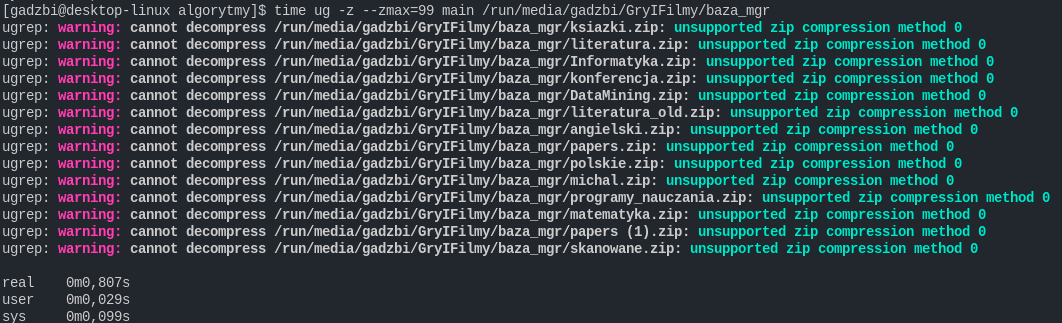
\includegraphics[width=0.7\textwidth]{./images/ugrep-errors.png}
\caption{Niepoprawne działanie programu ugrep dla archiwów pobranych z chmury}
\label{fig:ugrepErrors}
\end{figure}

Wiele z tych narzędzi nie działało poprawnie, gdy próbowaliśmy odczytać zawartość
archiwów. Przykładowo narzędzie ugrep (rys.\ref{fig:ugrepErrors}) nie rozpoznawało 
metody kompresji plików zip, co spowodowało, że nie nie otrzymaliśmy ani 
jednego rezultatu z programu. To powoduje, że narzędzie zostanie wykluczone z 
dalszej analizy.

Możliwym rozwiązaniem byłoby rozpakowanie wszystkich plików innym narzędziem, np.
7z. Takie podejście jednak znacznie komplikuje testowanie takiego rozwiązania.
Narzędzie powinno być w stanie samo rozpakować i wyszukać wszystkie frazy, które
chcemy wyszukać. Dodatkowo narzędzie powinno znajdować frazy zaraz po 
rozpakowaniu pliku, a nie po rozpakowaniu wszystkich archiwów zacząć przeszukiwać 
ich zawartość.

\begin{figure}[h]
\centering
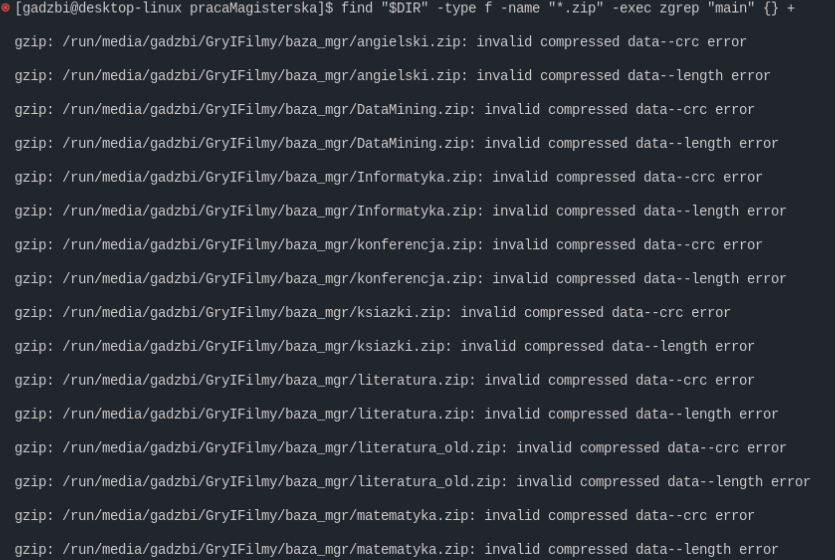
\includegraphics[width=0.7\textwidth]{./images/zgrep-errors.png}
\caption{Niepoprawne działanie programu zgrep z pomocą finda}
\label{fig:zgrepErrors}
\end{figure}

Kolejne z wymienionych narzędzi również nie spełnia wymagań. Zgrep nie pozwala
na rekurencyjne wyszukiwanie danych w folderach, w których znajdują się archiwa.
Nawet zastosowanie pomocniczego narzędzia find w celu wykonania zadania,
powoduje, że program nie jest w stanie przeskanować archiwów (rys. \ref{fig:zgrepErrors}).

Otrzymany błąd sugeruje, że długość danych w archiwum nie jest zgodna. Dodatkowo
mamy informacje o błędzie w wartości cyklicznej kontroli nadmiarowej CRC
(ang. \english{Cyclic Redundancy Check}). Ta wartość to system sum kontrolnych
pozwalający na wykrycie błędów zmagazynowanych danych.

\begin{figure}[h]
\centering
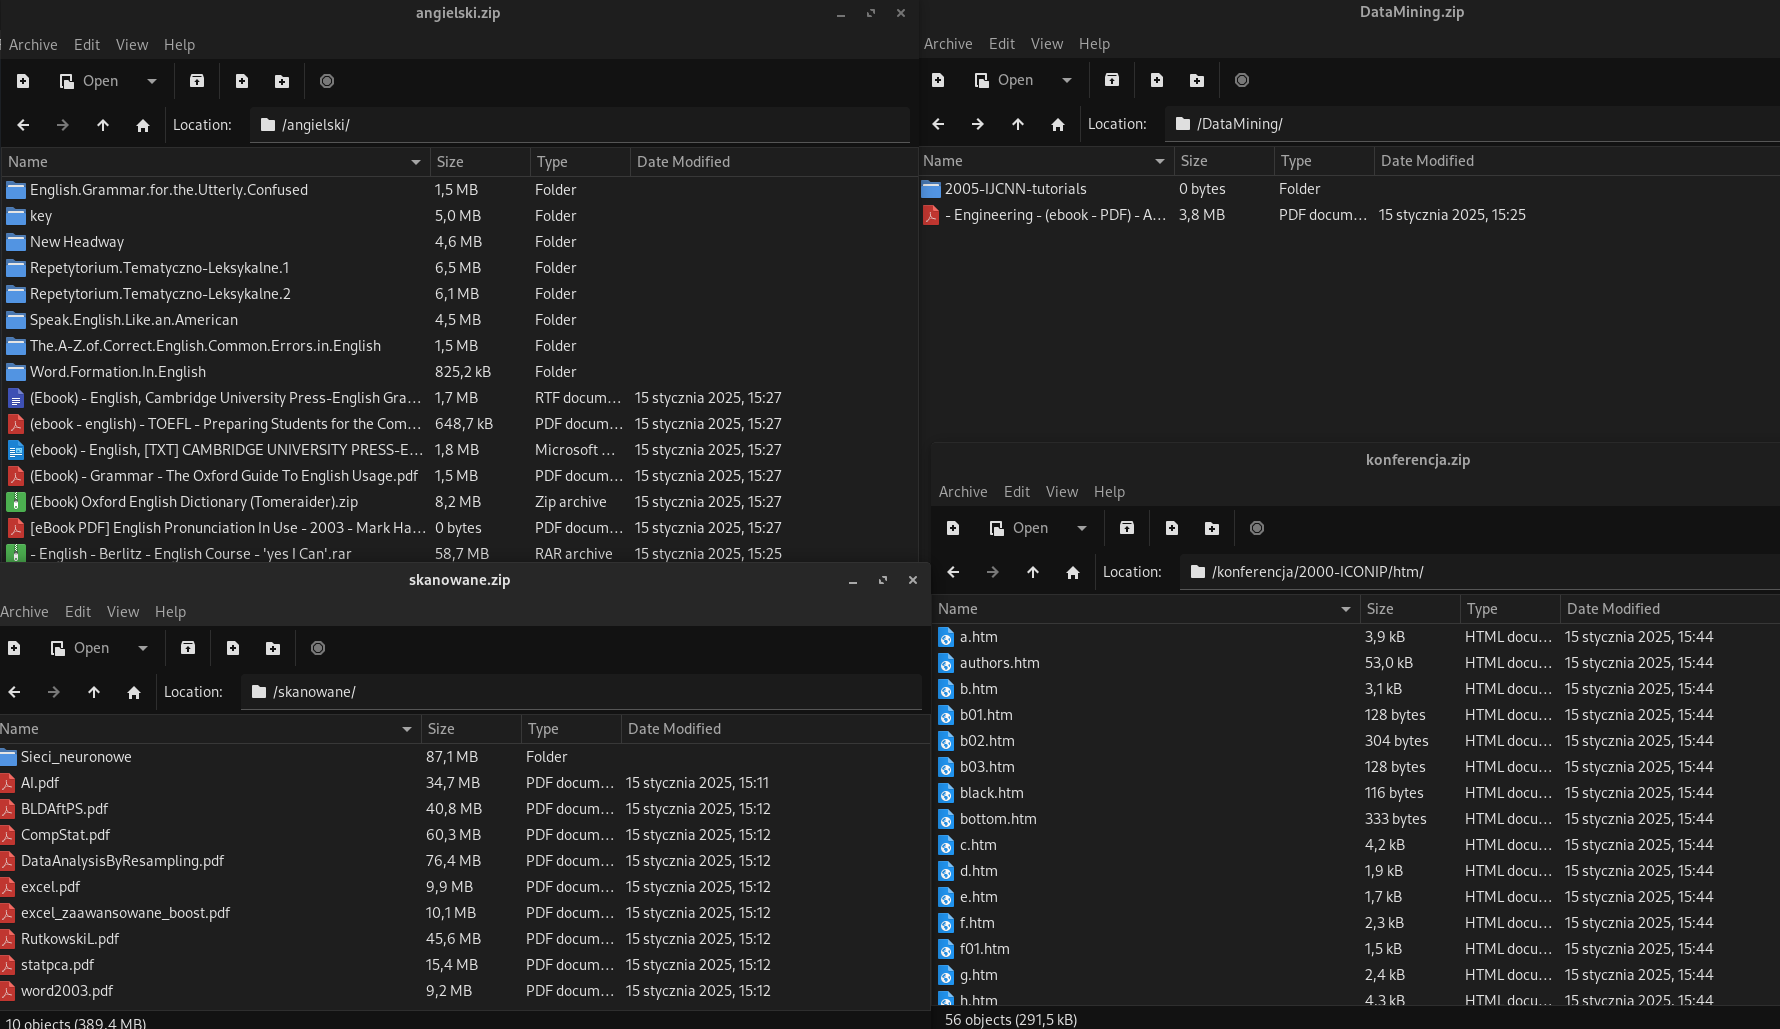
\includegraphics[width=0.7\textwidth]{./images/przykład-otwarcia-archiwów.png}
\caption{Przykład otwarcia archiwów przez program graficzny Engrampa}
\label{fig:engrampaExample}
\end{figure}

Archiwa jednak są możliwe do otworzenia przez program graficzny Engrampa \cite{bib:internet:EngrampaArchives}.
Choć wszystkie pliki zostały odczytane, oznacza to, że istnieje możliwość pozyskania
części zawartości (rys. \ref{fig:engrampaExample}).

Narzędzie graficzne nie będzie brane pod uwagę do badania, zostało jedynie podane
jako przykład poprawności archiwów.

\begin{figure}[h]
\centering
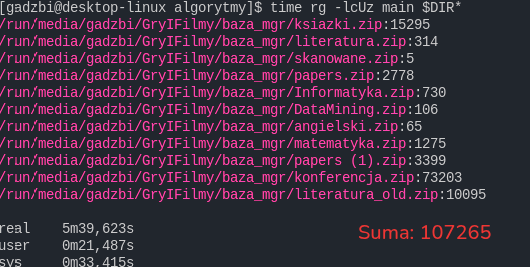
\includegraphics[width=0.7\textwidth]{./images/ripgrep-result-main.png}
\caption{Przykładowy rezultat wykonania komendy ripgrep ze zmierzonym czasem}
\label{fig:ripgrepResultMain}
\end{figure}

Narzędzie ripgrep pozwala na wyszukanie zawartości w archiwach i działa bardzo dobrze.
Narzędzie było w stanie wyszukać ogromną liczbę fraz "main" we wszystkich plikach \ref{fig:ripgrepResultMain}.
Narzędzie niestety nie posiada dokładnej lokalizacji, w której wystąpiło wyszukanie,
tylko jest w stanie wskazać miejsce w pliku skompresowanym konkretny bajt.
Taki rezultat nie mówi, w którym pliku znajdują się frazy, a jedynie może znaleźć 
kontekst w pliku lub podać ilość wystąpień.

Różnica ta jest znacząca w celu znalezienia frazy w konkretnym pliku. 
Implementacja gsearch pozwala na wyszukanie linii pliku w którym fraza się znajduje. 

\begin{figure}[h]
\centering
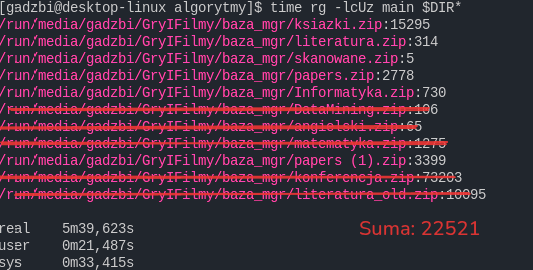
\includegraphics[width=0.7\textwidth]{./images/rgSkippedmain.png}
\caption{Liczba wystąpień "main" z pominięciem kilku archiwów}
\label{fig:ripgrepRemoveSkipped}
\end{figure}

Gdy odrzucimy pominięte przez gsearch archiwa \ref{fig:ripgrepRemoveSkipped},
widać liczba wystąpień w gsearch jest większy. Poniżej znajduje się zestawienie
ilości znalezionych wystąpień dla wszystkich archiwów przeszukiwanych przez rg,
pominiętych archiwów dla rg oraz pominiętych archiwów przeszukanych przez gsearch.

Należy wspomnieć, iż jedno wystąpienie dla ripgrepa to pojawienie się frazy
w danej linijce. W ten sam sposób liczone jest znalezienie wystąpienia w gsearch.
Implementacja gsearch nie posiada wrażliwości na wielkość liter, dlatego nie 
jest testowana

\begin{table}[h]
    \centering
    \begin{tabular}{|r|r|r|r|}
        \hline
        \textbf{Fraza (litery)} & \textbf{rg (wszystkie archiwa)} & \textbf{rg (pominięte)} &  \textbf{gsearch (pominięte)} \\
        \hline
        wan (3) & 34821 & 22951 & 20293 \\
        \hline
        main (4) & 107265 & 22521 & 23822 \\
        \hline
        window (6) & 16998 & 8251 & 9430 \\
        \hline
        analysis (8) & 3511 & 2168 & 1740 \\
        \hline
        book desc (9) & 6 & 3 & 3 \\
        \hline
        informatyka (11) & 1 & 1 & 5 \\
        \hline
        wInDoW (6) & 56760 & 20939 & 0 \\
        \hline
    \end{tabular}
    \caption{Tabela zestawienia wyników wyszukiwania dla działających programów}
    \label{tabela:iloscWyszukanDziekiProgramom}
\end{table}

Tabela \ref{tabela:iloscWyszukanDziekiProgramom} przedstawia wyniki ilości 
wystąpień fraz w zbiorze archiwów. Ponieważ implementacja gsearch nie potrafi
przeszukać określonych archiwów, zdecydowano się na zestawienie rezultatów
ripgrepa ze wszystkich archiwów, oraz z tego samego zbioru archiwów pominiętych. 

\begin{figure}[ht]
    \centering
    \begin{tikzpicture}[scale=1.50]
        \begin{axis}[
        xlabel=Długość słowa,
        ylabel=Ilość znalezionych linii]
        \addplot[color=orange,mark=x]coordinates{
            (3,22951)
            (4,22521)
            (6,8251)
            (8,2168)
            (9,3)
            (11,3)
        };
        \addplot[color=blue,mark=x]coordinates{
            (3,20293)
            (4,23822)
            (6,9430)
            (8,1740)
            (9,3)
            (11,5)
        };
        \end{axis}
    \end{tikzpicture}
    \caption{Wykres wystąpień linii z frazami w zależności od długości liter w słowie }
    \label{fig:wykresPorównaniaIlosciWystapień}
\end{figure}

Ostatni wiersz pokazuje jakie znaczenie ma wyszukiwanie po wielkości liter 
(tab. \ref{tabela:iloscWyszukanDziekiProgramom}). Program ripgrep posiada 
możliwość ignorowania wielkości liter czego nie robi program gsearch. Jeżeli
nie znamy dokładnej wielkości liter frazy, to może to spowodować brak 
znalezienia frazy (rys. \ref{fig:wykresPorównaniaIlosciWystapień}). 


Program ripgrep nie jest w stanie znaleźć zawartości archiwów zagnieżdżonych w
innych archiwach. Rozwiązuje ten problem gsearch i pozwala na wyszukanie 
znalezienie konkretnego pliku w którym fraza się znajduje.

\section{Porównanie prędkości wyszukiwania programów}

Porównane zostaną programy, które pozwoliły uzyskać oczekiwany rezultat i są to
ripgrep oraz implementowany gsearch. 
Porównanie szybkości wyszukiwania zostanie wykonane na pomniejszonym zbiorze,
aby porównanie czasów było sprawdzane na tym samym zbiorze, gdzie oba programy
są w stanie odczytać z nich dane.

\begin{figure}[ht]
    \centering
    \begin{tikzpicture}[scale=1.50]
        \begin{axis}[
        xlabel=Długość słowa,
        ylabel=Czas znalezienia słów (s)]
        \addplot[color=orange,mark=*,error bars/.cd, y dir=both, y explicit]coordinates{
(3,0.6393700976599999)+=(0,0.007651709374308371)-=(0,0.007651709374308371)
(4,0.69975840454)+-(0,0.02174176683244841)
(6,0.6708412953200001)+-(0,0.04320545697230668)
(8,0.76563712796)+-(0,0.041486089097604)
(9,0.62396489284)+-(0,0.007851351947769116)
(11,0.6782059222)+-(0,0.04570502275958309)
        };
        \addplot[color=blue,mark=*,error bars/.cd, y dir=both, y explicit]coordinates{
(3,20.081044353359996)+-(0,0.4395975771554202)
(4,19.78817344134)+-(0,0.20913605765611032)
(6,19.25416691472)+-(0,0.21635912584660782)
(8,18.88328445046)+-(0,0.19096399774593745)
(9,18.916769088339997)+-(0,0.5162741966007814)
(11,18.5046544439)+-(0,0.17920383136563042)
        };
        \end{axis}
    \end{tikzpicture}
    \caption{Wykres czasów znalezienia fraz w zależności od długości liter dwóch programach}
    \label{fig:wykresPorównaniaCzasówWyszukań}
\end{figure}

Prędkości wyszukiwania danych za pomocą ripgrepa są znacznie większe, niż te
za pomocą gsearch (rys. \ref{fig:wykresPorównaniaCzasówWyszukań}). Wynika to z
tego, że ripgrep wykonuje wyszukiwania z wykorzystaniem kilku wątków. Dodatkowo 
program rg ładuje pliki prosto do pamięci, natomiast program gsearch rozpakowuje
zawartość pliku archiwum do folderu, a następnie czyta zawartość każdego pliku.

Takie podejście było konieczne, gdyż Golang ma wbudowane większe ograniczenia w 
proces alokowania danych i tego ile danych może przechowywać w pamięci w danym momencie.

Wykorzystanie innego języka dającego większą swobodę w manipulowaniu pamięcią 
dałoby lepsze czasy wykonania, jednak wykorzystanie języka niskopoziomowego,
wiąże się z większym czasem implementacji algorytmów oraz trudniejszym procesem
analizowania błędów.

Dodatkowo ripgrep wykorzystuje operacje SIMD (ang. \english{Single Instruction, Multiple Data}),
czyli wykonanie wielu porównania w ciągu jednego cyklu. Te operacje znacznie
przyspieszają wykonanie wyszukiwania.

Ripgrep dla fraz o długości 3 lub mniejszych używa algorytmu Teddy. Ten algorytm
pozwala na załadowanie całej frazy do rejestru XMM i wykonania bitowego 
porównania małej frazy z zawartością danych przeszukiwanych.

\subsection{Wykorzystanie profilowania do oczytania charakterystki programu}

\begin{figure}[h]
  \centering
  \begin{lstlisting}
f, _ := os.Create("profile.pprof")
pprof.StartCPUProfile(f)
defer pprof.StopCPUProfile()
  \end{lstlisting}
  \caption{Dodanie profilowania do programu gsearch}
  \label{fig:code:profilerGsearch}
\end{figure}

Można również sprawdzić charakterystkę programu gsearch dodając kod na początek 
wykonania programu (rys. \ref{fig:code:profilerGsearch}). Wykonanie programu na
słowie "informatyka" utworzy plik profile.pprof. Ten plik można przejrzeć w 
przeglądarce wcześniej wykorzystując komendę \textbf{go tool pprof -http=localhost:8090 profile.pprof}.

\begin{figure}[h]
\centering
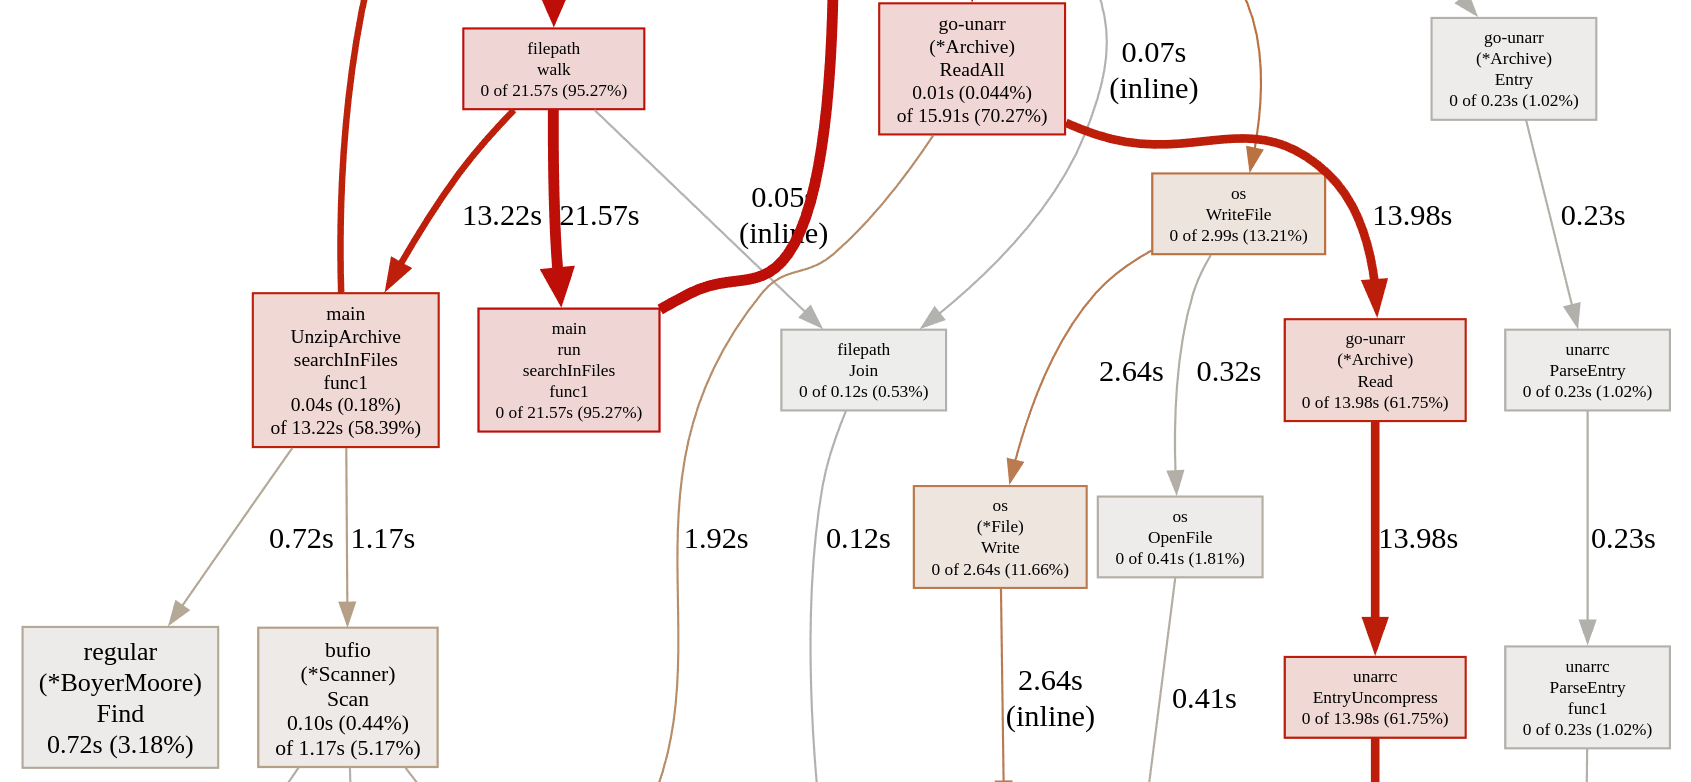
\includegraphics[width=0.7\textwidth]{./images/profiler1.png}
\caption{Przykład grafu wykonań funkcji w gsearch}
\label{fig:profilerGsearch1}
\end{figure}

Po wykonaniu komendy przeglądarce otworzy się widok na graf programu (rys. \ref{fig:profilerGsearch1}).
Graf jest bardzo skomplikowany do analizy w przypadku, gdy wykorzystujemy rekursje w programie do
przeszukiwania folderów i rozpakowywania zawartości.

Można zauważyć, że większość czasu programu wykorzystywana jest na operacje 
ekstrakcji archiwów i czytania archiwów. Sam algorytm przeszukujący (dolny lewy 
róg rys. \ref{fig:profilerGsearch1}) wykonuje się jedynie 0.72 sekundy.

\begin{figure}[h]
\centering
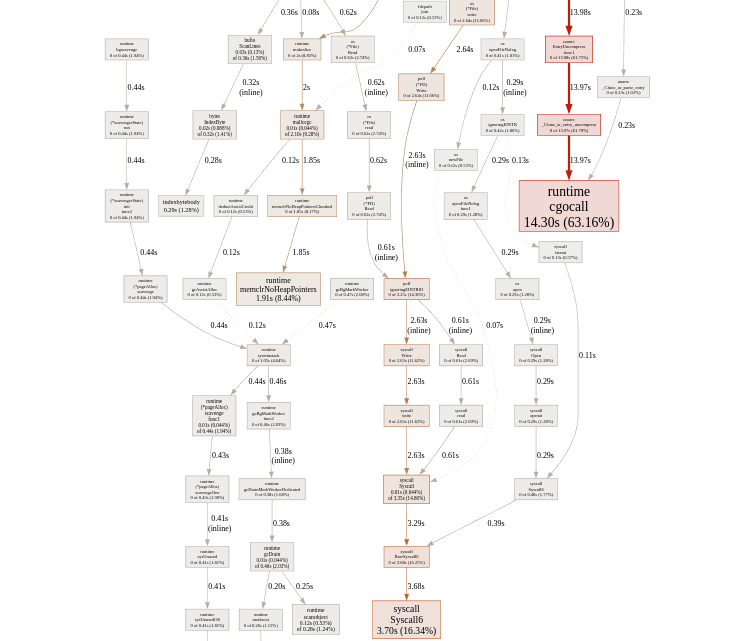
\includegraphics[width=0.7\textwidth]{./images/profiler2.png}
\caption{Zdjęcie grafu funkcji "runtime cgocall" oraz "syscall6"}
\label{fig:profilerGsearch2}
\end{figure}

Głównym ograniczeniem prędkości działania jest czas odczytywania zawartości z plików.
Funkcje "runtime cgocall" oraz "syscall6" stanowią znaczną część czasu
wykonywania programu (rys. \ref{fig:profilerGsearch2}), które wykonują operacje
odczytu zawartości treści z dysku. % Badania

% TODO

\chapter{Podsumowanie}

%\begin{itemize}
%\item Jaki problem rozwiązałæm?
%\item Jak ten problem rozwiązałæm?
%\item Jakie są dobre i słabe strony mojego rozwiązania?
%\item Czy mogę sformułować jakieś rekomendacje?
%\end{itemize}

\begin{itemize}
\item syntetyczny opis wykonanych prac
\item wnioski
\item możliwość rozwoju, kontynuacji prac, potencjalne nowe kierunki
\item Czy cel pracy zrealizowany? 
\end{itemize}

 % Podsumowanie

\backmatter

%\bibliographystyle{plplain}  % bibtex
%\bibliography{biblio/biblio} % bibtex
\printbibliography           % biblatex
\addcontentsline{toc}{chapter}{Bibliografia}

\begin{appendices}

    % TODO
    % \chapter{Dokumentacja techniczna}
 % dokumentacja techniczna

    % TODO
    \chapter{Spis skrótów i symboli}

\begin{itemize}
\item[GC] ang. \english{Garbage Collector} - Zbieracz śmieci w programie 
%\item[DNA] kwas deoksyrybonukleinowy (ang. \english{deoxyribonucleic acid})
%\item[MVC] model -- widok -- kontroler (ang. \english{model--view--controller}) 
%\item[$N$] liczebność zbioru danych
%\item[$\mu$] stopnień przyleżności do zbioru
%\item[$\mathbb{E}$] zbiór krawędzi grafu
%\item[$\mathcal{L}$] transformata Laplace'a 
\end{itemize} % Spis skrótów i symboli

    % TODO
    % \chapter{Lista dodatkowych plików, uzupełniających tekst pracy (jeżeli dotyczy)} 

% W systemie do pracy dołączono dodatkowe pliki zawierające:
% \begin{itemize}
% \item źródła programu,
% \item zbiory danych użyte w~eksperymentach,
% \item film pokazujący działanie opracowanego oprogramowania lub zaprojektowanego i wykonanego urządzenia,
% \item itp.
% \end{itemize}
 % Lista dodatkowych plików, uzupełniających tekst pracy – jeżeli dotyczny, w przecinym razie – zakomentuj!

    \listoffigures
    \addcontentsline{toc}{chapter}{Spis rysunków}
    \listoftables
    \addcontentsline{toc}{chapter}{Spis tabel}

\end{appendices}

\end{document}


%% Finis coronat opus.

